\documentclass[aspectratio=169,10pt,xcolor=table]{beamer}
\usepackage[utf8]{inputenc}
\usepackage[T1]{fontenc}
\usepackage[spanish,es-tabla,es-nodecimaldot,es-noquoting]{babel}
\usepackage{lmodern}
\usepackage{amsmath}
\usepackage{booktabs}
\usepackage{tabularx}
\usepackage{array}
\usepackage{graphicx}
\usepackage{microtype}

\graphicspath{{../latex/img/}}

% ==============================================================================
% PALETA SOBRIA UNSAAC (COHERENTE CON INFORME Y FIGURAS DEL PROYECTO)
% ==============================================================================
\definecolor{azulInst}{HTML}{1B4965}
\definecolor{azulSuave}{HTML}{EDF4F8}
\definecolor{grisTexto}{HTML}{334155}
\definecolor{grisSuave}{HTML}{F8FAFC}
\definecolor{bordeSuave}{HTML}{CBD5E1}
\definecolor{naranjaAcc}{HTML}{D96B43}
\definecolor{verdeAcc}{HTML}{1F8A70}

% ==============================================================================
% CONFIGURACIÓN VISUAL DE BEAMER (LIMPIA, 16:9, SIN SOBRECARGA)
% ==============================================================================
\usetheme{default}
\usecolortheme{default}
\setbeamertemplate{navigation symbols}{}
\setbeamersize{text margin left=0.65cm, text margin right=0.65cm}

\setbeamercolor{normal text}{fg=black!90,bg=white}
\setbeamercolor{structure}{fg=azulInst}
\setbeamercolor{frametitle}{fg=white,bg=azulInst}
\setbeamercolor{title}{fg=azulInst}
\setbeamercolor{subtitle}{fg=grisTexto}
\setbeamercolor{block title}{fg=white,bg=azulInst}
\setbeamercolor{block body}{fg=black!90,bg=azulSuave}
\setbeamercolor{item}{fg=azulInst}

\setbeamertemplate{itemize item}{\color{azulInst}\rule[0.1ex]{0.7ex}{0.7ex}}
\setbeamertemplate{itemize subitem}{\color{azulInst}$\triangleright$}

% Encabezado de diapositiva compacto y centrado (títulos de 1 línea)
\setbeamerfont{frametitle}{size=\large,series=\bfseries}
\setbeamertemplate{frametitle}{%
  \nointerlineskip%
  \begin{beamercolorbox}[wd=\paperwidth,ht=0.64cm,dp=0.24cm,leftskip=0.65cm,rightskip=0.65cm]{frametitle}%
    \usebeamerfont{frametitle}\insertframetitle%
  \end{beamercolorbox}%
  \nointerlineskip%
  {\color{naranjaAcc}\hrule height 1.2pt}%
}

% Pie de página discreto
\setbeamertemplate{footline}{%
  {\color{bordeSuave}\hrule height 0.5pt}%
  \begin{beamercolorbox}[wd=\paperwidth,ht=0.34cm,dp=0.14cm,leftskip=0.65cm,rightskip=0.65cm]{footline}%
    \scriptsize\color{grisTexto}%
    \textbf{\color{azulInst}UNSAAC · FIEEIM} · Visión por Computador (2026-II)%
    \hfill%
    Grupo N.\ 9 · Estudio CNN en HAM10000%
    \hfill%
    \textbf{\color{azulInst}\insertframenumber{} / \inserttotalframenumber}%
  \end{beamercolorbox}%
}

% Macro auxiliar para tarjetas limpias sin bordes gruesos
\newcommand{\tarjetainf}[2]{%
  \begin{beamercolorbox}[wd=\linewidth,rounded=false,sep=5pt,leftskip=2pt,rightskip=2pt]{block body}%
    {\footnotesize\bfseries\color{azulInst}#1}\\[2pt]%
    {\scriptsize\color{black!88}#2}%
  \end{beamercolorbox}%
}

\title[Clasificación Dermatoscópica (HAM10000)]{Evaluación Comparativa de Tres Arquitecturas CNN para Clasificación de Lesiones Cutáneas Pigmentadas mediante Dermatoscopia (HAM10000)}
\author{Grupo N.\ 9 — UNSAAC}
\date{2026}

\begin{document}

% ==============================================================================
% DIAPOSITIVA 1: PORTADA
% ==============================================================================
\begin{frame}[plain]
  \vspace*{-0.25cm}
  \begin{beamercolorbox}[wd=\paperwidth,ht=1.25cm,dp=0.28cm,leftskip=0.65cm,rightskip=0.65cm]{frametitle}
    \centering
    {\normalsize\bfseries UNIVERSIDAD NACIONAL DE SAN ANTONIO ABAD DEL CUSCO}\\[2pt]
    {\footnotesize Facultad de Ingeniería Eléctrica, Electrónica, Informática y Mecánica · E.\ P.\ de Ingeniería Informática y de Sistemas}
  \end{beamercolorbox}
  {\color{naranjaAcc}\hrule height 1.8pt}

  \vspace{0.14cm}
  \begin{columns}[c,onlytextwidth]
    \begin{column}{0.19\textwidth}
      \centering
      
\includegraphics[height=3.25cm,keepaspectratio]{escudo.png}
    \end{column}
    \begin{column}{0.79\textwidth}
      \begin{beamercolorbox}[wd=\linewidth,sep=6pt]{block body}
        {\scriptsize\bfseries\color{grisTexto} VISIÓN POR COMPUTADOR (2026-II) · EXPOSICIÓN FINAL DE INVESTIGACIÓN}\\[3pt]
        {\Large\bfseries\color{azulInst} Evaluación Comparativa de Tres Arquitecturas CNN para Clasificación de Lesiones Cutáneas Pigmentadas mediante Dermatoscopia (HAM10000)}\\[4pt]
        {\small\color{grisTexto} Transferencia de aprendizaje, partición sin fuga por lesión, análisis de robustez con mitigación espacial y eficiencia en GPU NVIDIA GTX 1650}
      \end{beamercolorbox}
      \vspace{0.14cm}
      {\small\color{black!90}
        \textbf{\color{azulInst}Docente:} Mg.\ Hans Harley Ccacyahuillca Bejar \quad\textbar\quad
        \textbf{\color{azulInst}Equipo:} Grupo N.\ 9
      }
    \end{column}
  \end{columns}

  \vspace{0.12cm}
  \begin{center}
    \small
    \renewcommand{\arraystretch}{1.18}
    \begin{tabularx}{0.88\textwidth}{@{}>{\centering\arraybackslash}p{0.08\textwidth}>{\raggedright\arraybackslash}X>{\centering\arraybackslash}p{0.22\textwidth}@{}}
      \toprule
      \rowcolor{azulSuave} \textbf{\color{azulInst}N.\textsuperscript{o}} & \textbf{\color{azulInst}Presentado por} & \textbf{\color{azulInst}Código Institucional} \\ \midrule
      1 & Choquenaira Quispe, Noe Franklin & 133962 \\
      2 & Porroa Sivana, Yeni Ruth & 120893 \\
      3 & Colque Galindo, Jean Franco & 193109 \\
      \bottomrule
    \end{tabularx}
  \end{center}
  \vspace{0.12cm}
  {\centering\scriptsize\color{grisTexto} Cusco -- Perú · 2026 \par}
  \vspace{0.18cm}
\end{frame}

% ==============================================================================
% DIAPOSITIVA 2: PROBLEMA, HAM10000 Y DESBALANCE 58.3:1
% ==============================================================================
\begin{frame}{1. Tarea dermatoscópica, 7 clases reales y desbalance (58.3:1)}
  \begin{columns}[c,onlytextwidth]
    \begin{column}{0.37\textwidth}
      \centering
      {\scriptsize\bfseries\color{azulInst} 7 categorías clínicas de HAM10000}\\[3pt]
      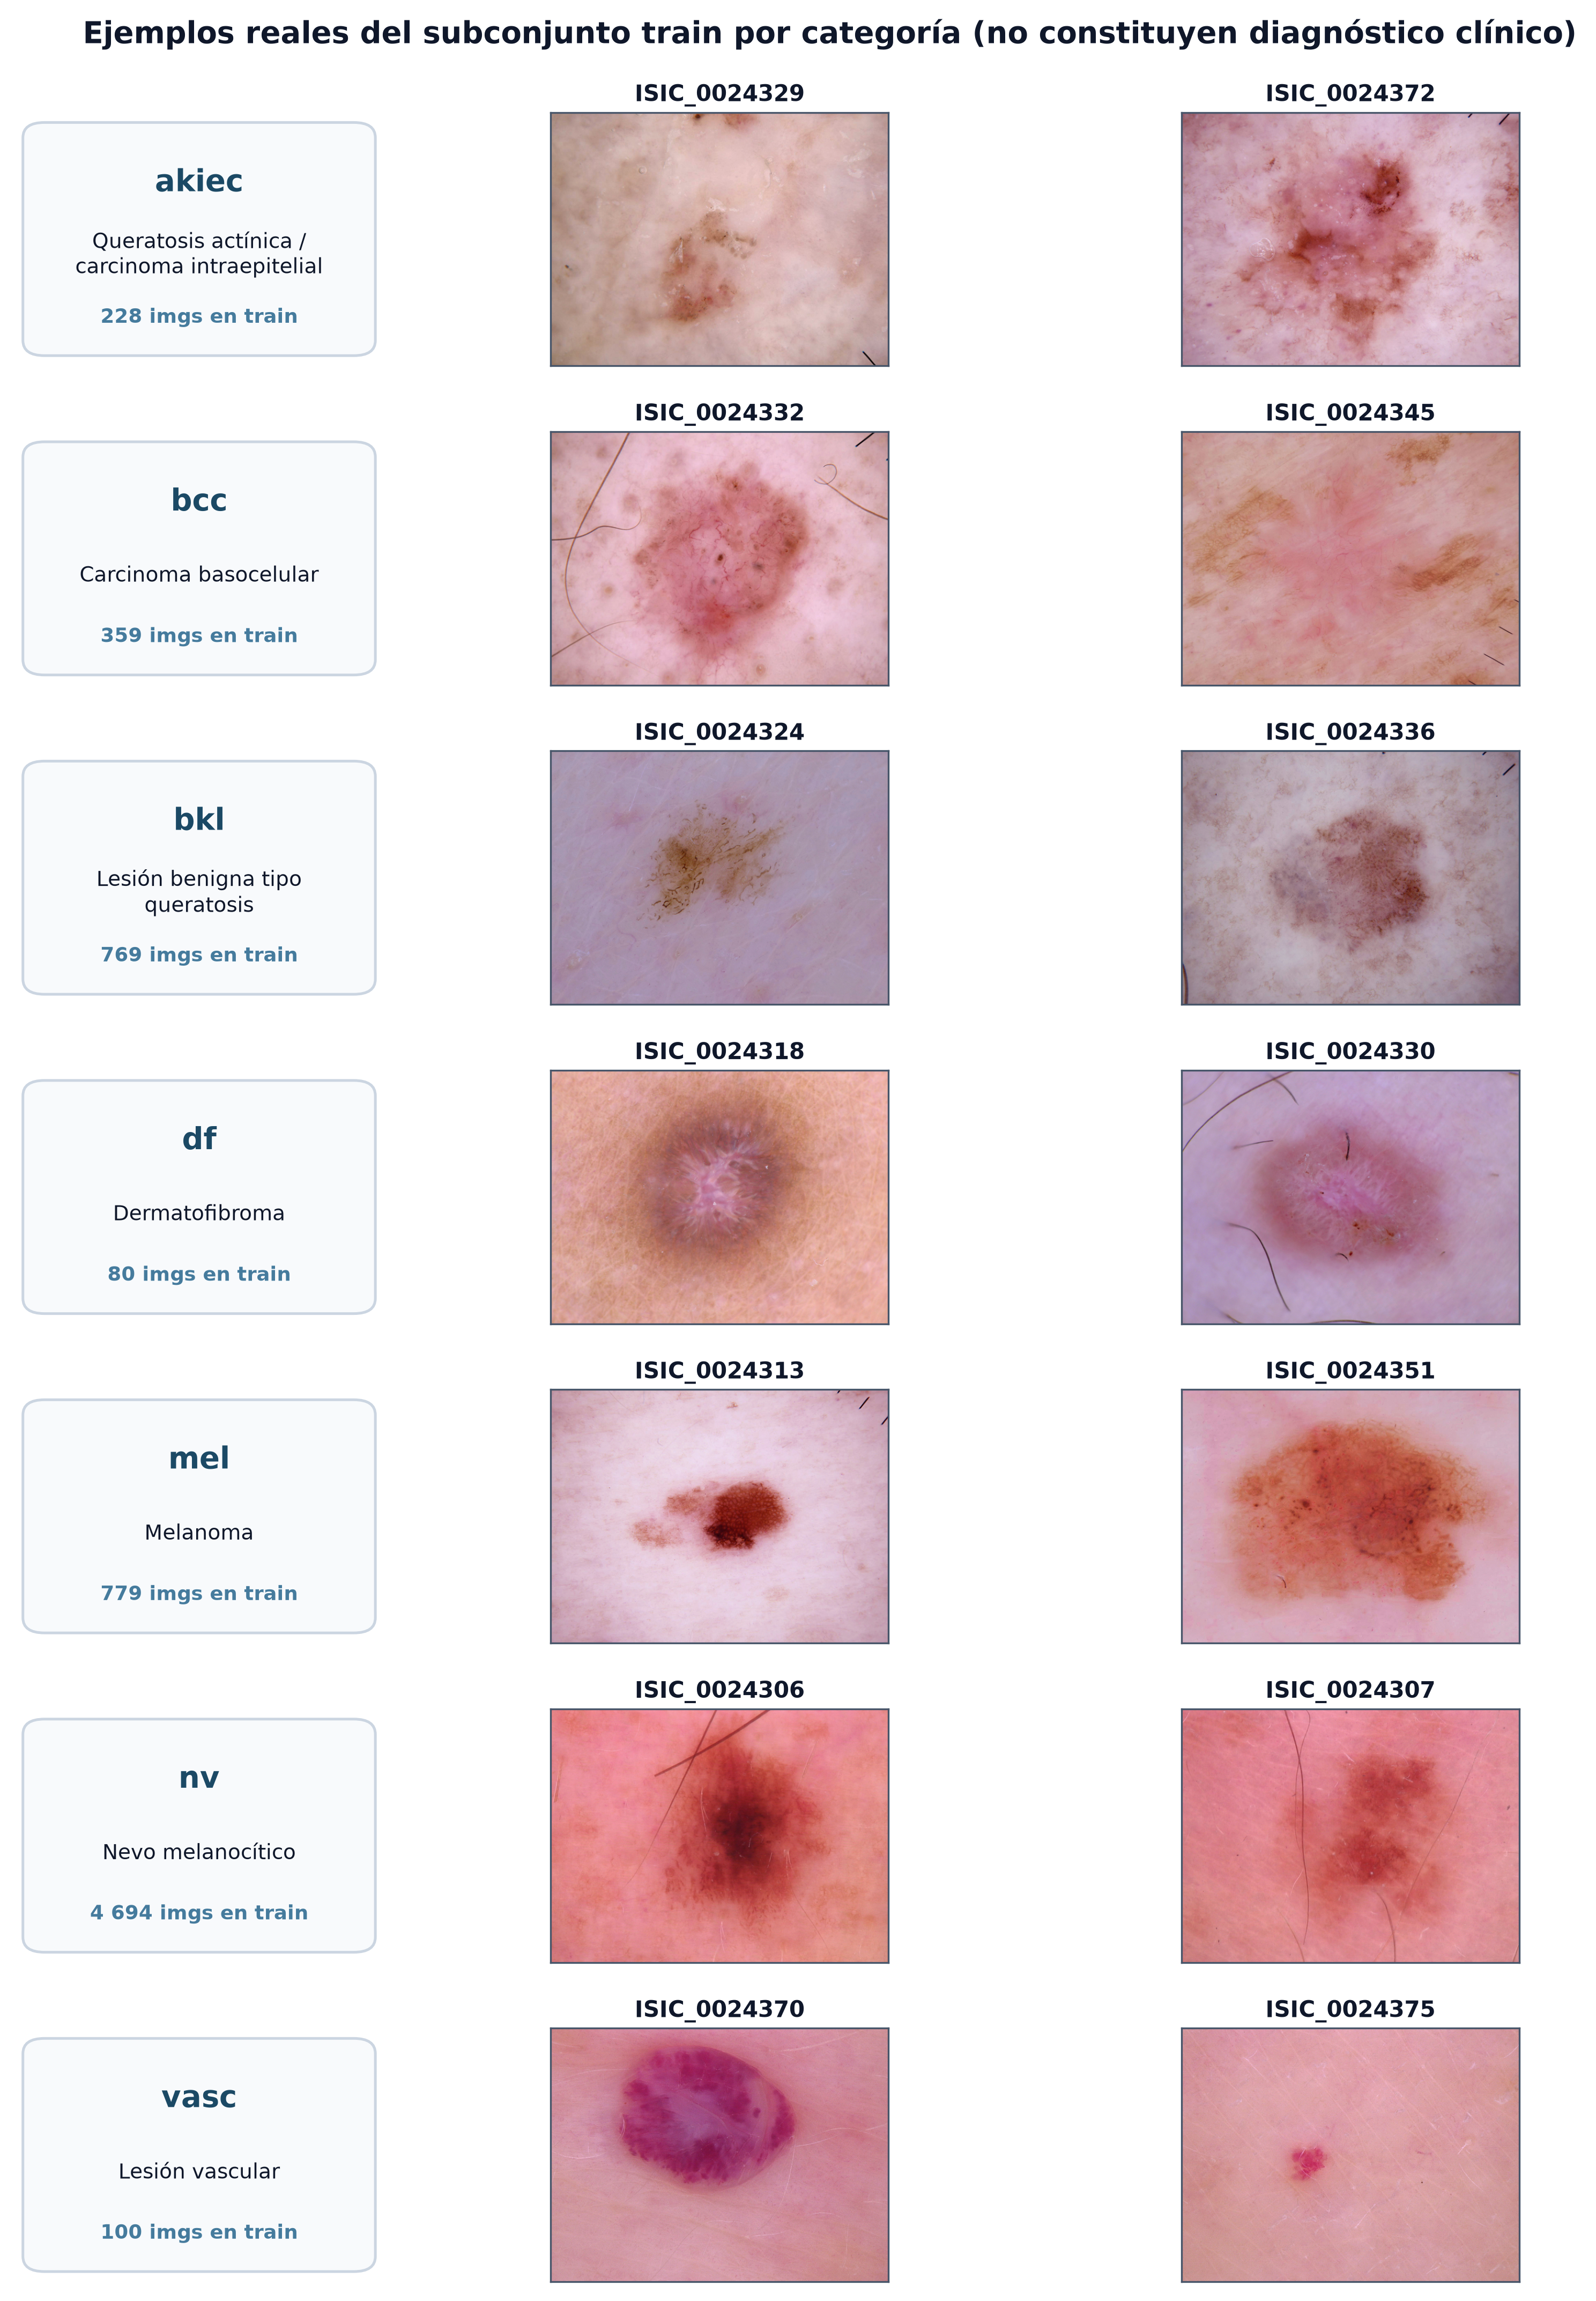
\includegraphics[height=5.25cm,keepaspectratio]{03_muestras.png}
    \end{column}
    \begin{column}{0.61\textwidth}
      \tarjetainf{Colección HAM10000 y desbalance extremo (58.3:1)}{%
        \textbf{10\,015} imágenes dermatoscópicas ($600\times 450$) de \textbf{7\,470} lesiones únicas. La clase \texttt{nv} concentra el \textbf{66.95\%} (6\,705) frente a \texttt{df} (\textbf{1.15\%}, 115) y \texttt{vasc} (\textbf{1.42\%}, 142).}
      \vspace{0.10cm}
      \centering
      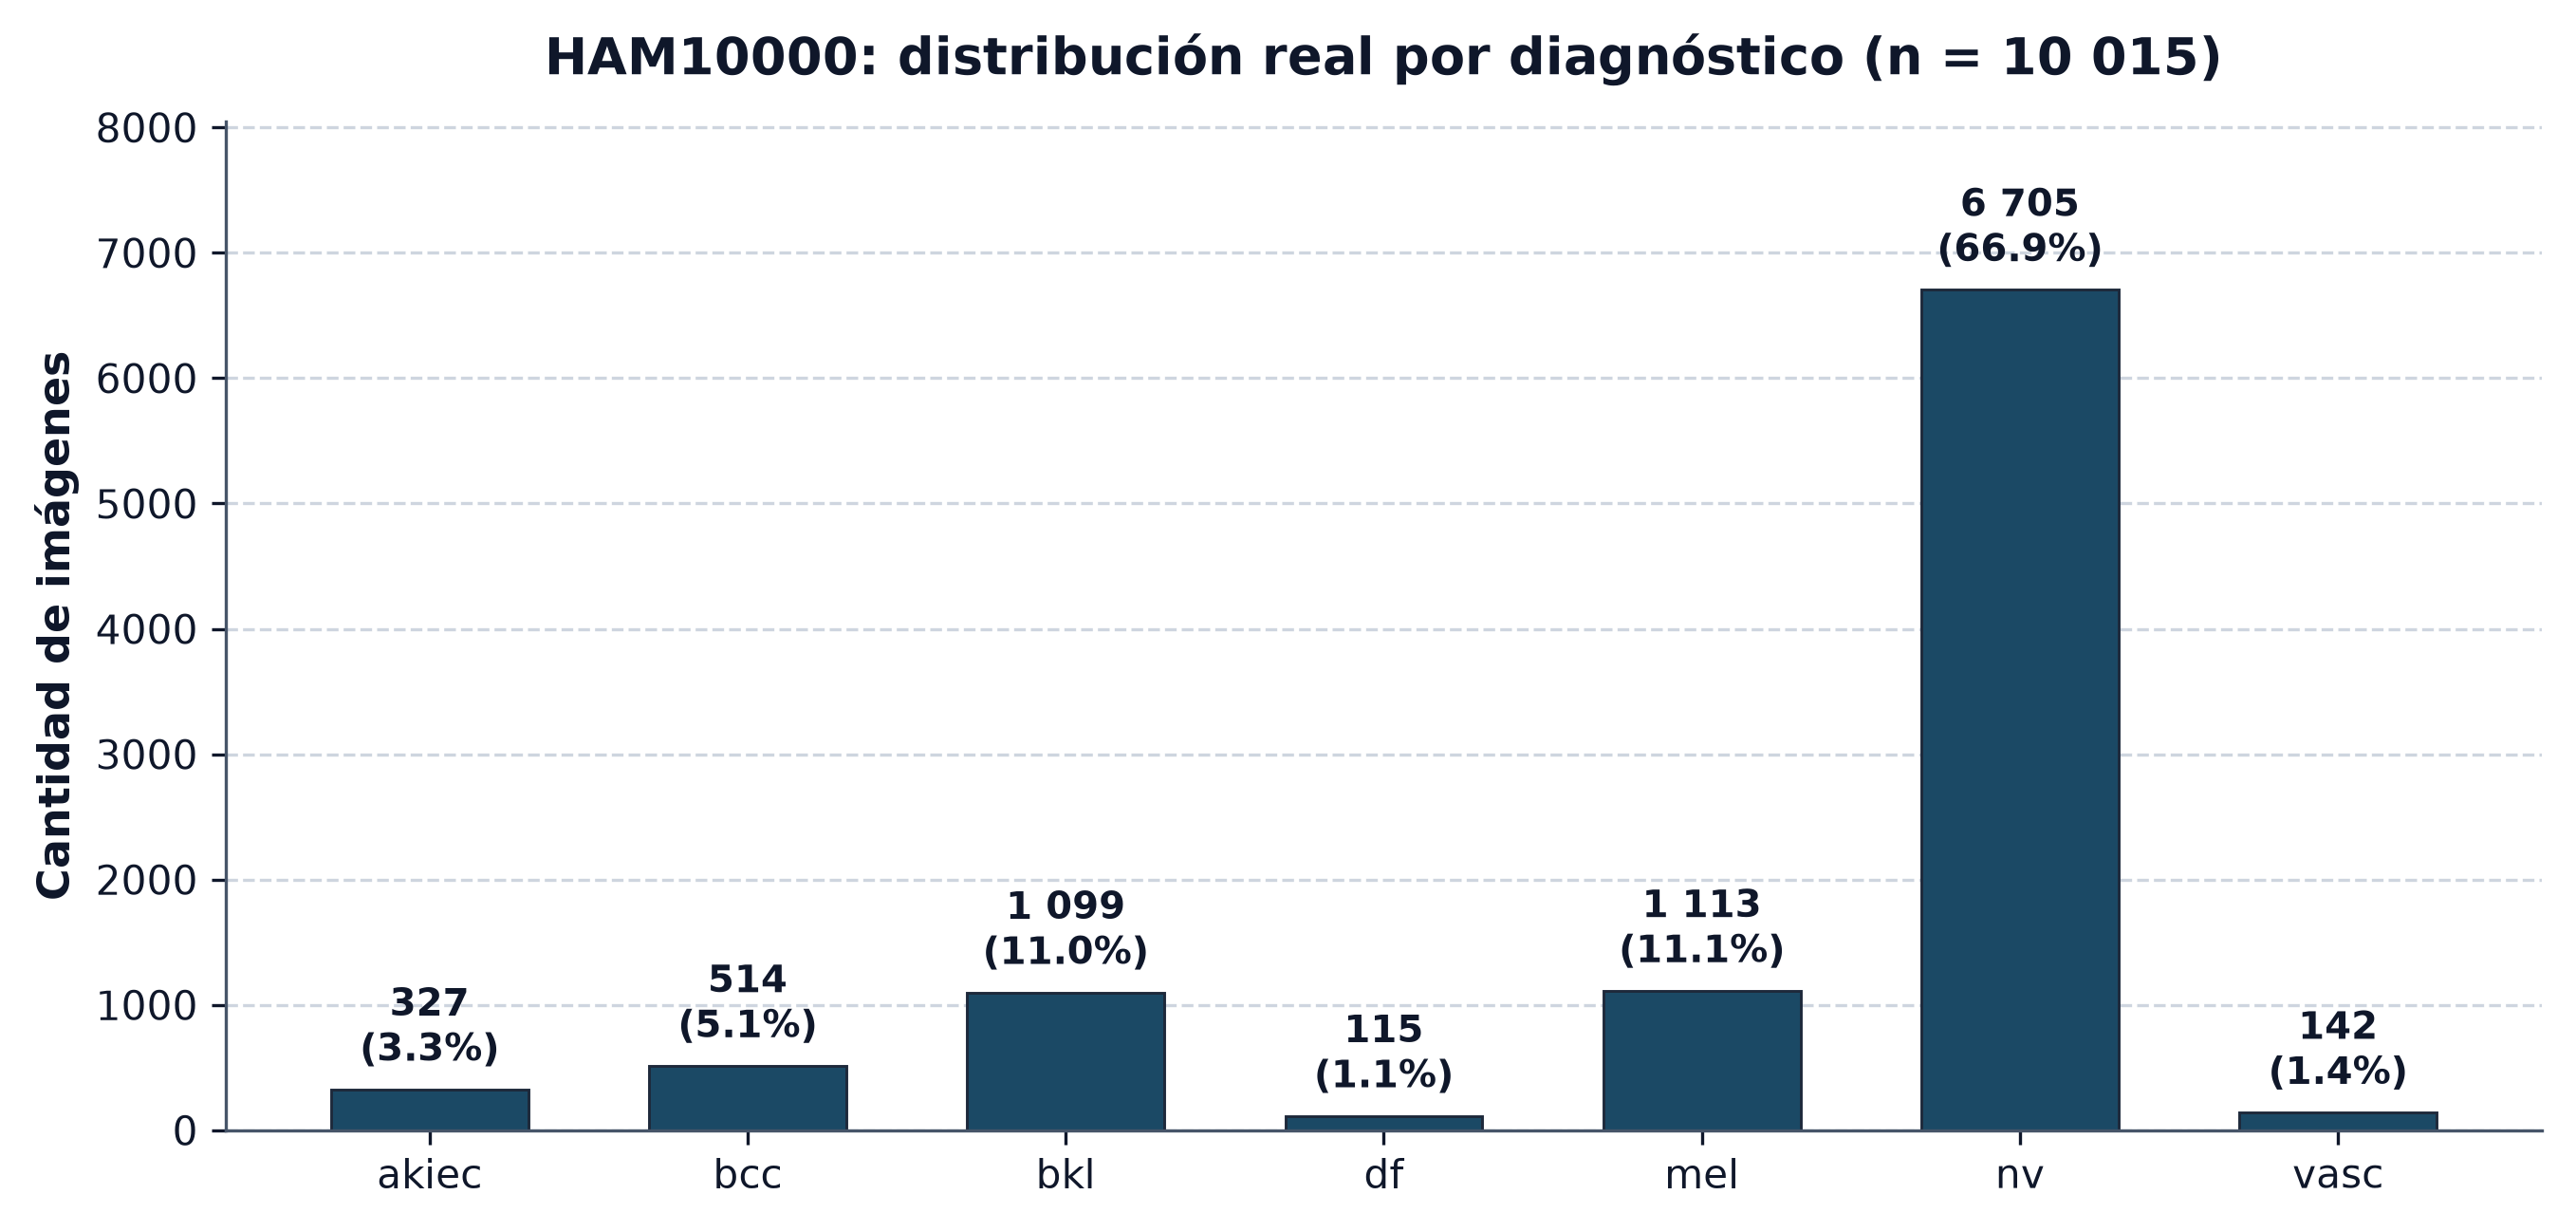
\includegraphics[width=\linewidth,height=2.70cm,keepaspectratio]{01_clases.png}
      \vspace{0.08cm}
      \begin{beamercolorbox}[wd=\linewidth,sep=4pt]{block body}
        {\scriptsize\bfseries\color{azulInst}Desafío visual y enfoque metodológico:}\\[2pt]
        {\scriptsize
        $\bullet$ \textbf{Fronteras difusas:} Dificultad visual intrínseca entre \texttt{mel}, \texttt{nv} y \texttt{bkl}.\\
        $\bullet$ \textbf{Fuga por lesión:} Múltiples tomas por lesión exigen agrupar por \texttt{lesion\_id}.\\
        $\bullet$ \textbf{Métricas:} \textit{Accuracy} trivial engañosa ($>66\%$). Se priorizan \textbf{Macro Prec.}, \textbf{Macro F1}, \textbf{Recall de melanoma} y \textbf{AUC OVR}.}
      \end{beamercolorbox}
    \end{column}
  \end{columns}
\end{frame}

% ==============================================================================
% DIAPOSITIVA 3: AUDITORÍA SHA-256 Y SPLIT SIN FUGA
% ==============================================================================
\begin{frame}{2. Auditoría criptográfica SHA-256 y partición fija sin fuga}
  \centering
  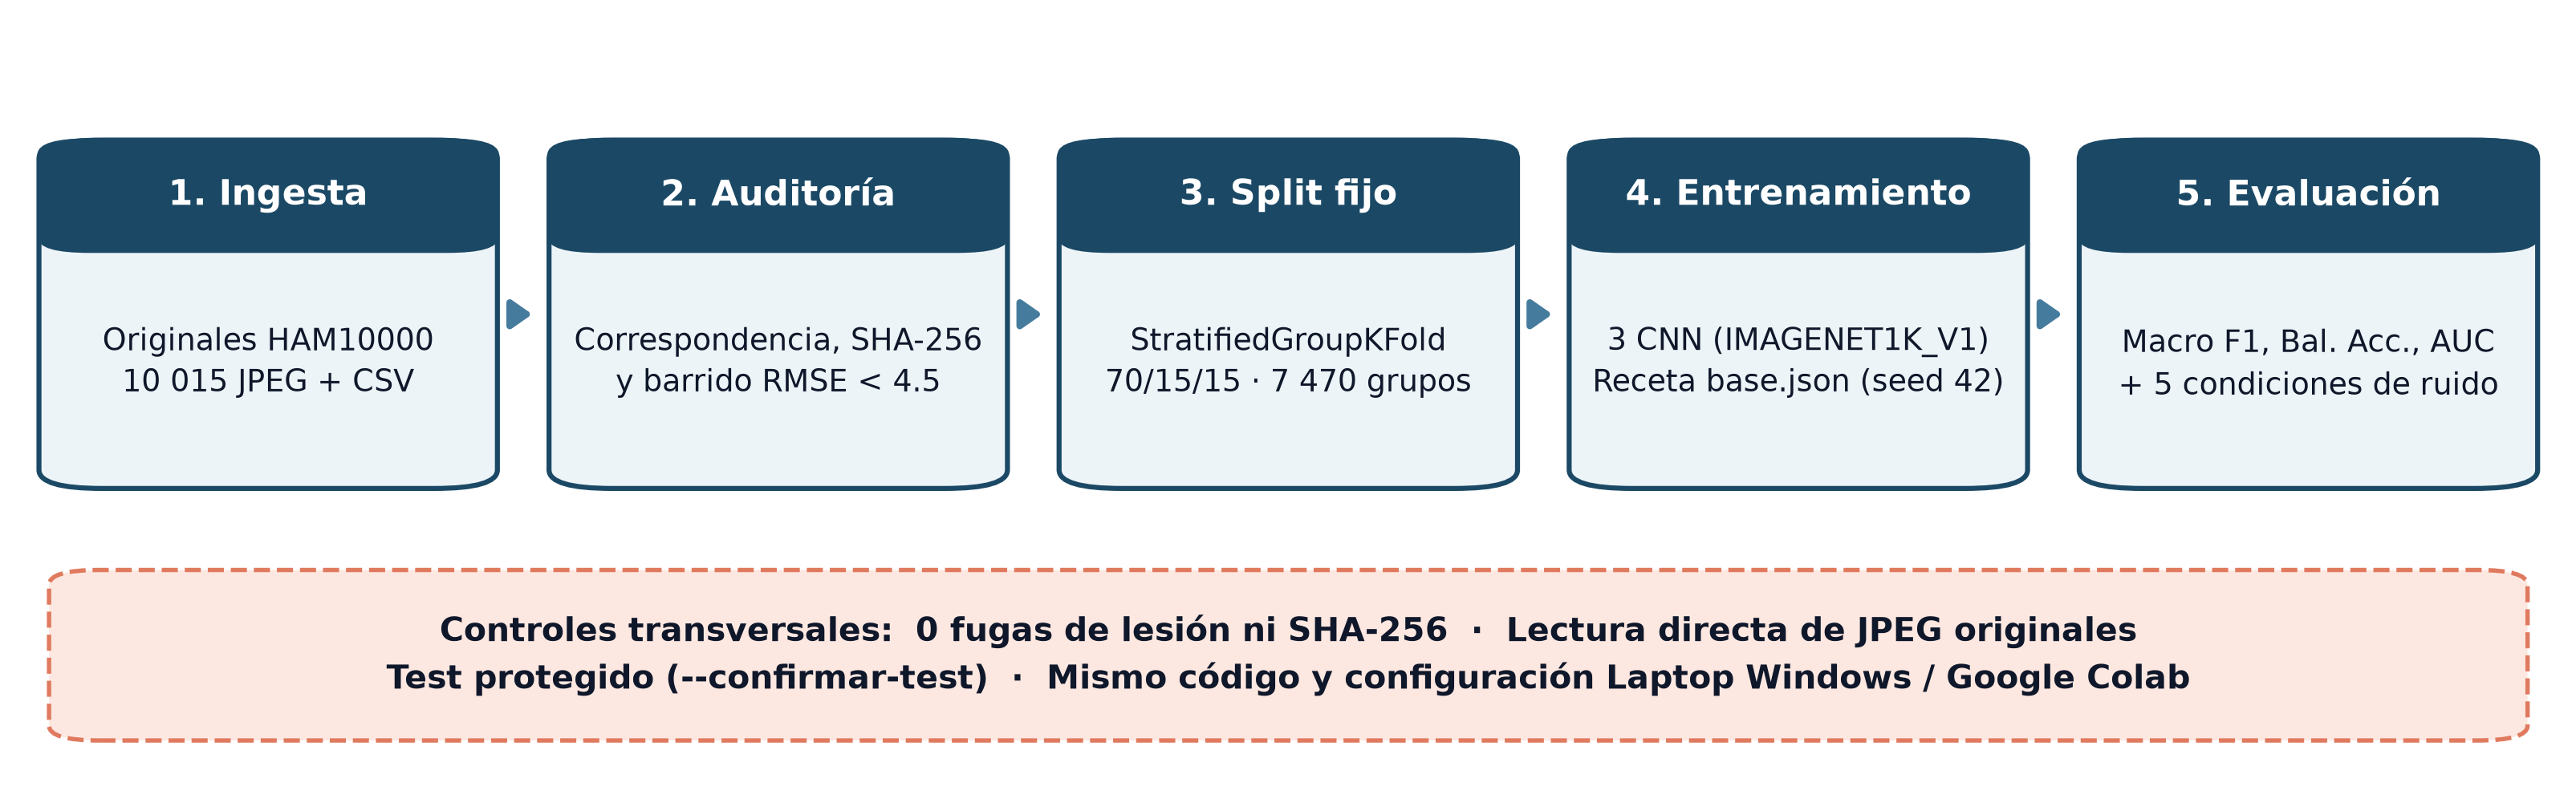
\includegraphics[width=0.98\textwidth,height=1.95cm,keepaspectratio]{10_pipeline.png}

  \vspace{0.10cm}
  \begin{columns}[c,onlytextwidth]
    \begin{column}{0.51\textwidth}
      \centering
      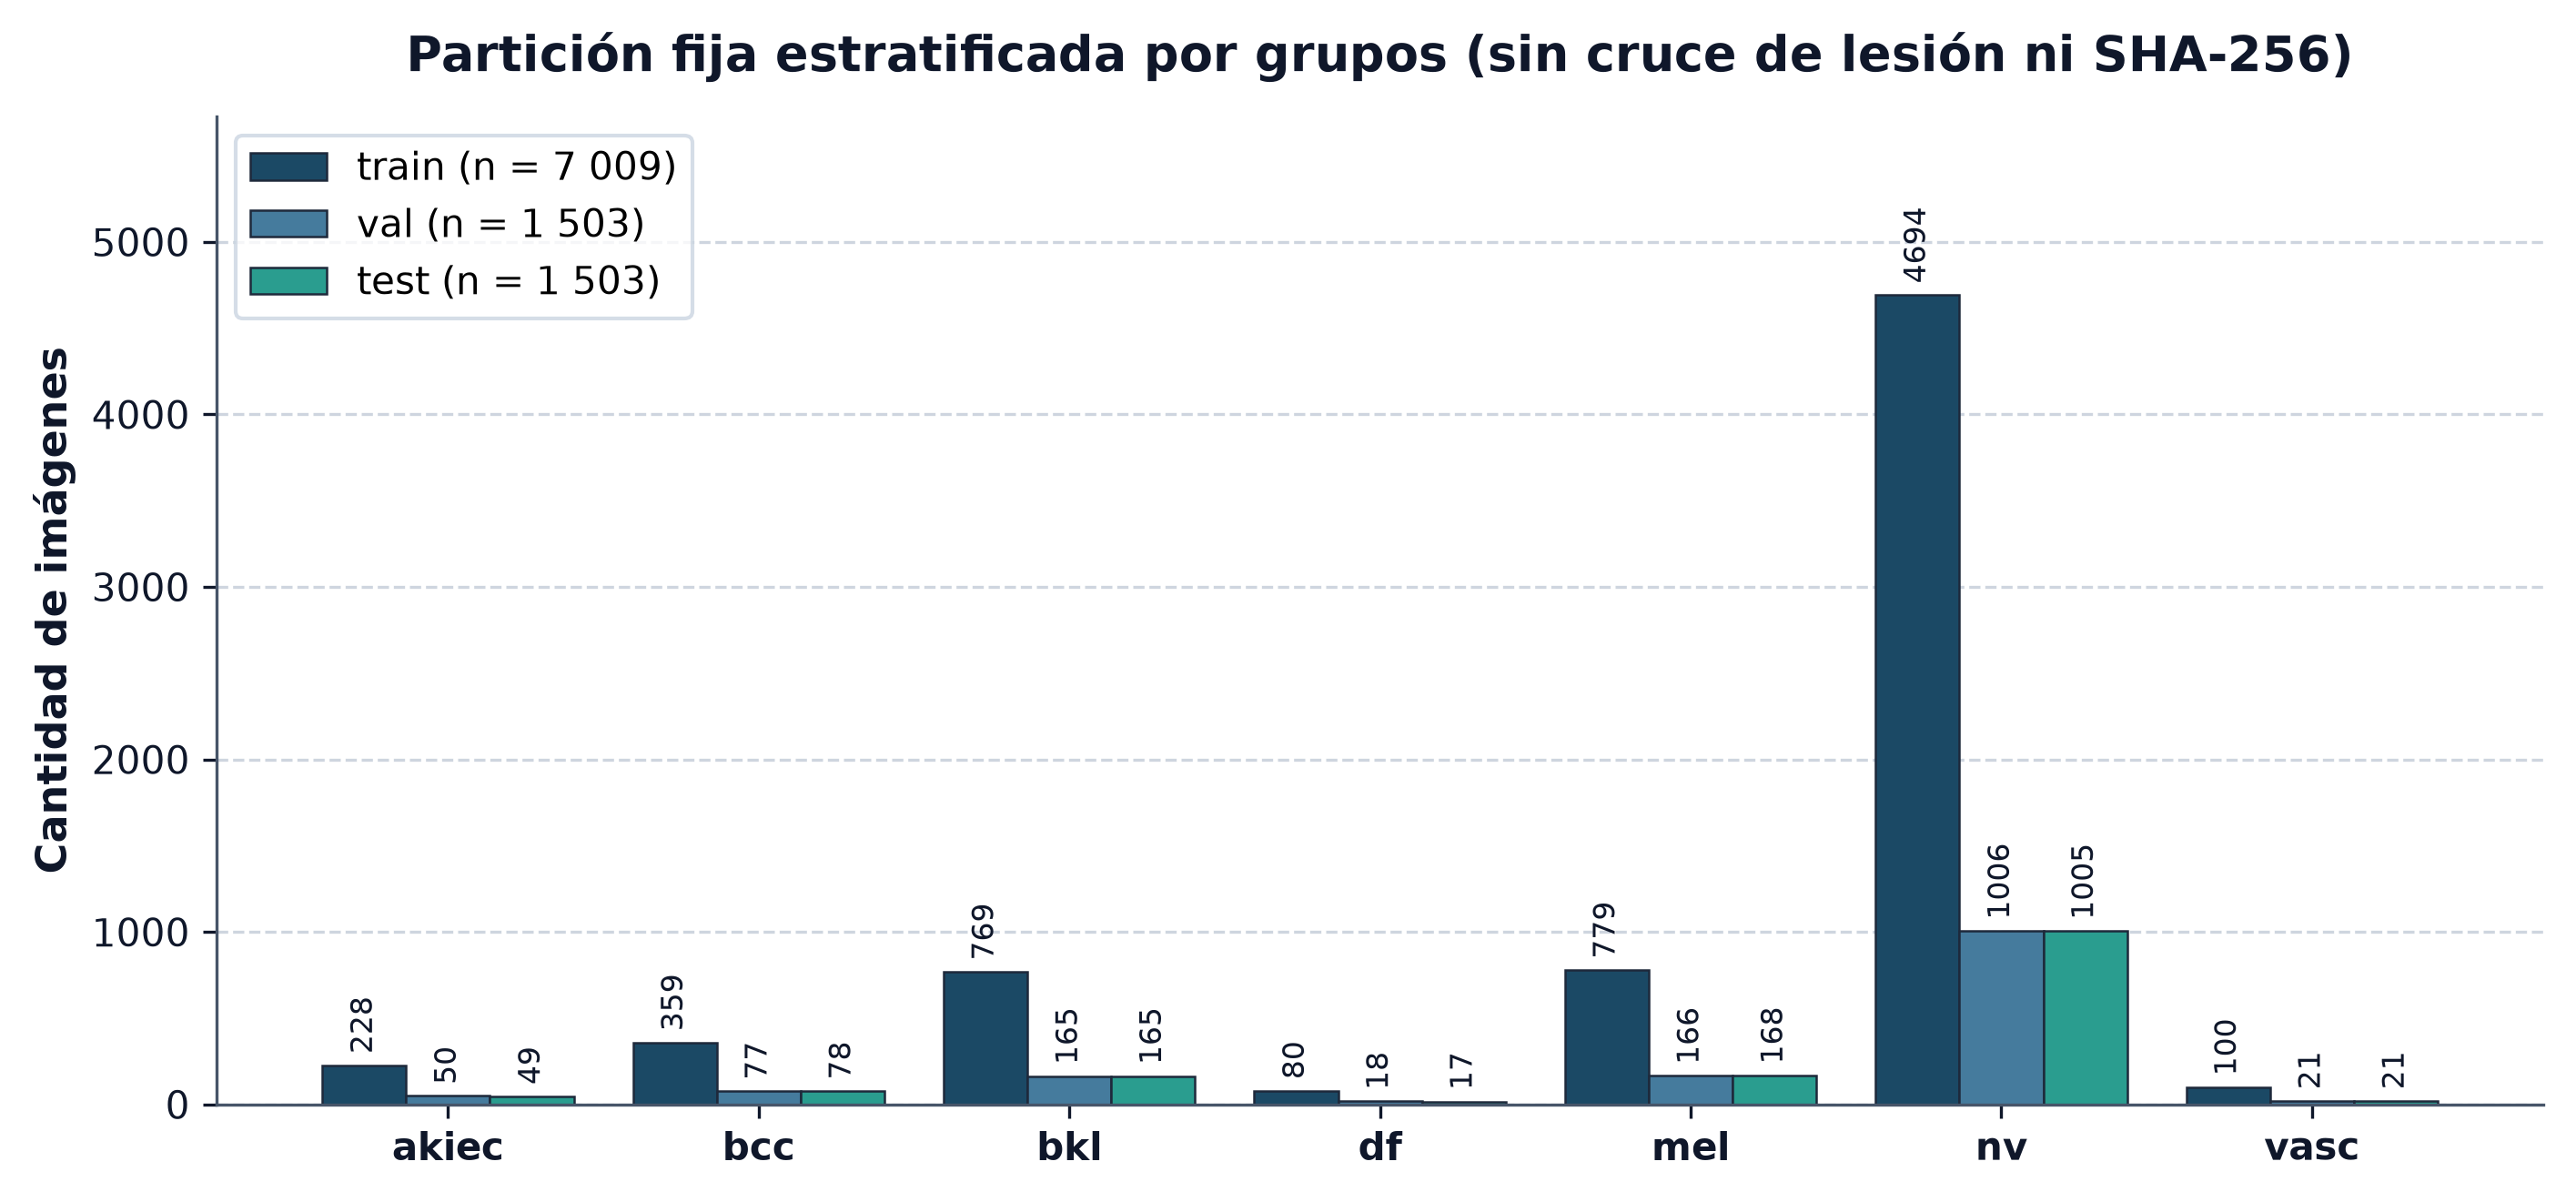
\includegraphics[width=\linewidth,height=3.80cm,keepaspectratio]{04_split.png}
    \end{column}
    \begin{column}{0.47\textwidth}
      \begin{beamercolorbox}[wd=\linewidth,sep=6pt]{block body}
        {\footnotesize\bfseries\color{azulInst}Resultados de auditoría y partición}
        \vspace{3pt}
        \scriptsize
        \begin{itemize}\setlength{\itemsep}{3pt}
          \item \textbf{Depuración de origen:} consolidación de \texttt{part\_1} + \texttt{part\_2} y remoción de copias redundantes (5.20 $\to$ 2.71 GiB).
          \item \textbf{Duplicados exactos:} 2 pares SHA-256 idénticos detectados (\texttt{HAM\_0002300} y \texttt{HAM\_0001895}) y mantenidos juntos.
          \item \textbf{Casi-duplicados:} \textbf{0 pares} entre lesiones distintas con $\mathrm{RMSE}<4.5$ en miniaturas $16\times 12$ (verificación de sesión).
          \item \textbf{Split \texttt{StratifiedGroupKFold(20)} (seed 42):}
                \texttt{train} \textbf{7\,009} (70\%) · \texttt{val} \textbf{1\,503} (15\%) · \texttt{test} \textbf{1\,503} (15\%).
          \item \textbf{0 fugas:} intersección nula de \texttt{lesion\_id}, grupo o SHA-256 (\texttt{split\_sha256: 583779fb...}).
        \end{itemize}
      \end{beamercolorbox}
    \end{column}
  \end{columns}
\end{frame}

% ==============================================================================
% DIAPOSITIVA 4: PREPROCESAMIENTO ISOTRÓPICO Y AUMENTO DETERMINISTA
% ==============================================================================
\begin{frame}{3. Preprocesamiento isotrópico y aumento determinista}
  \centering
  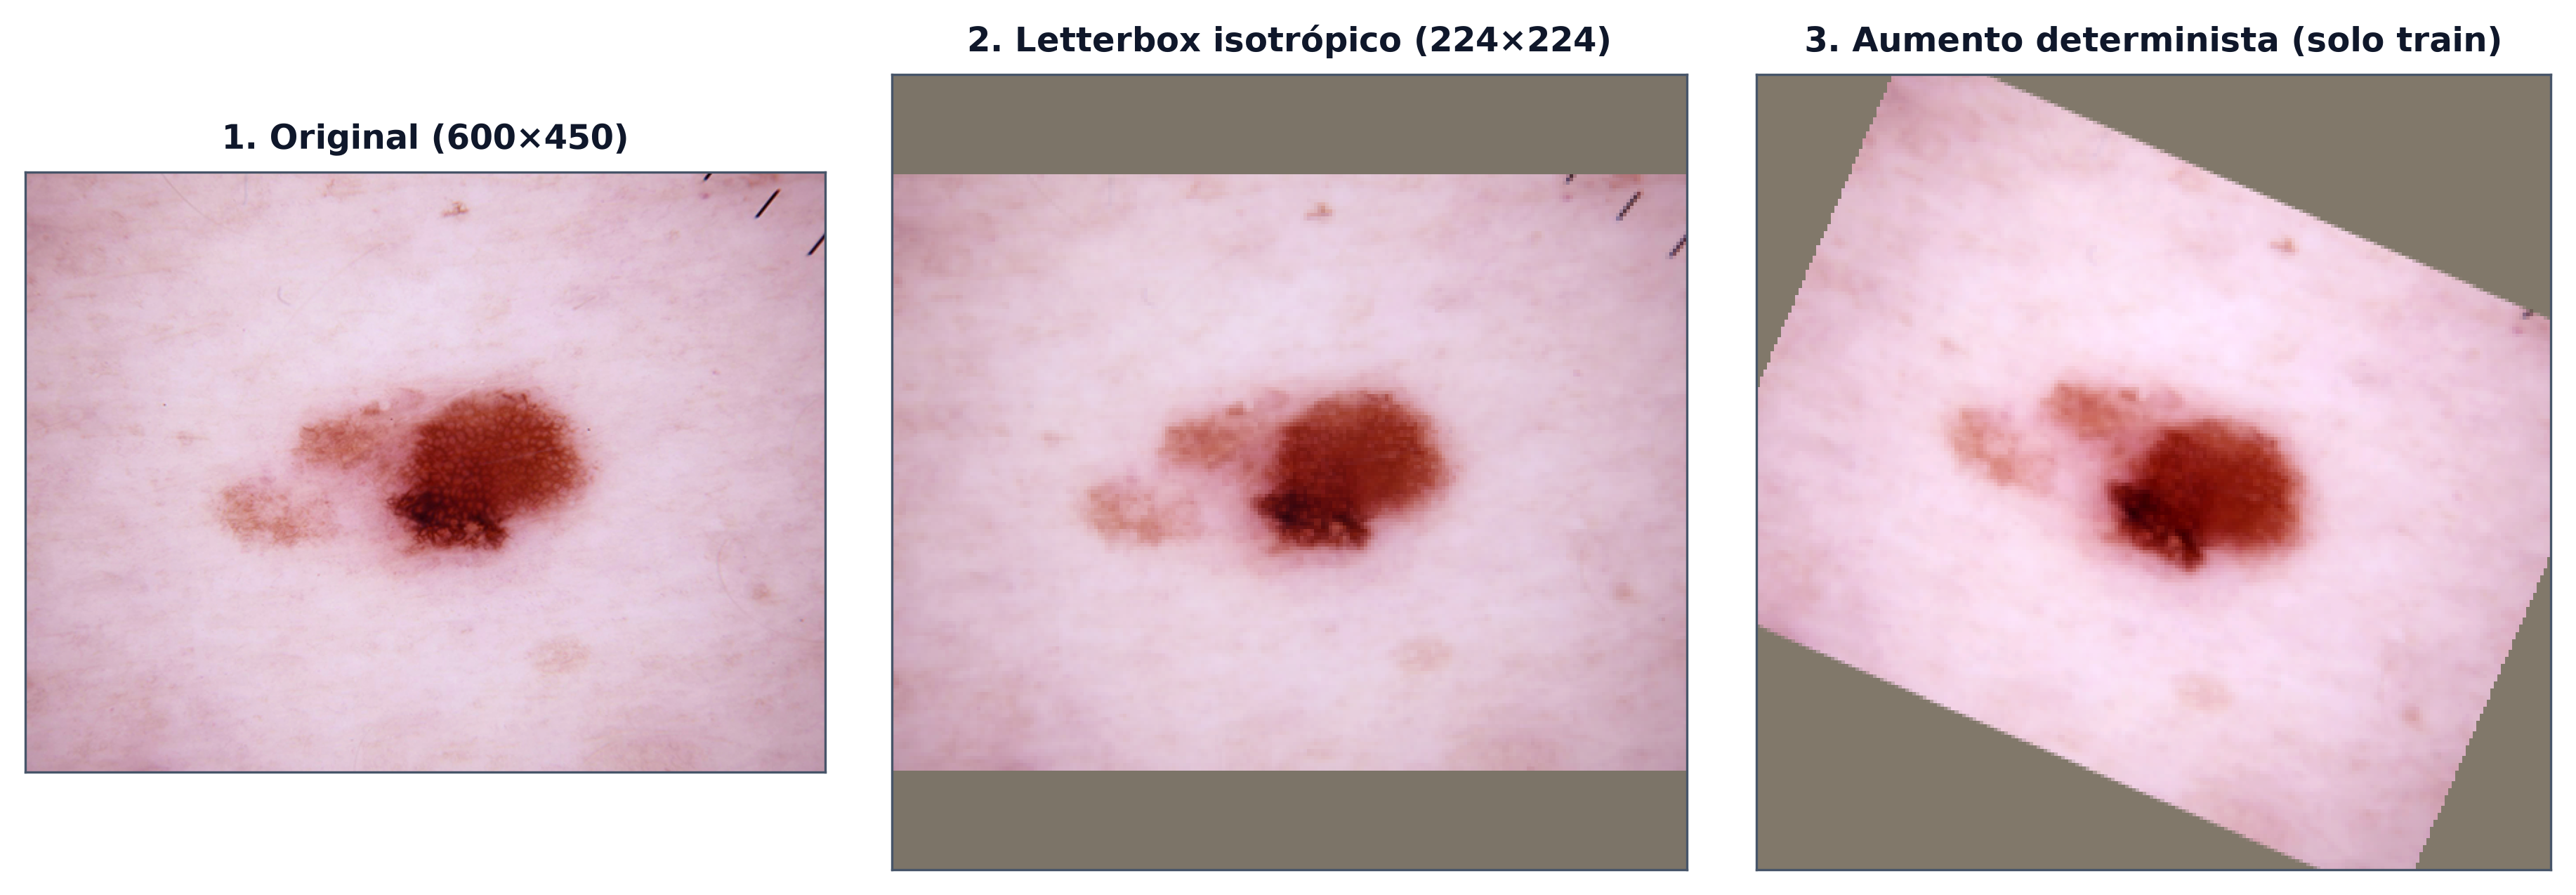
\includegraphics[width=0.98\textwidth,height=3.15cm,keepaspectratio]{08_preprocesamiento.png}

  \vspace{0.12cm}
  \begin{columns}[T,onlytextwidth]
    \begin{column}{0.49\textwidth}
      \begin{beamercolorbox}[wd=\linewidth,sep=5pt]{block body}
        {\footnotesize\bfseries\color{azulInst}Pipeline geométrico (\texttt{train / val / test})}
        \vspace{2pt}
        \scriptsize
        \begin{itemize}\setlength{\itemsep}{2pt}
          \item Lectura directa de JPEG originales ($600\times 450$) en RGB (orientación EXIF corregida).
          \item \textbf{Letterbox isotrópico $224\times 224$:} preserva la relación de aspecto sin distorsión anatómica ni recorte periférico.
          \item Normalización por canal con ImageNet ($\mu=[0.485,0.456,0.406]$, $\sigma=[0.229,0.224,0.225]$).
        \end{itemize}
      \end{beamercolorbox}
    \end{column}
    \begin{column}{0.49\textwidth}
      \begin{beamercolorbox}[wd=\linewidth,sep=5pt]{block body}
        {\footnotesize\bfseries\color{azulInst}Aumento determinista (solo \texttt{train})}
        \vspace{2pt}
        \scriptsize
        \begin{itemize}\setlength{\itemsep}{2pt}
          \item \textbf{Sin fuga en test:} aumento aplicado exclusivamente al conjunto de entrenamiento.
          \item Volteo H/V ($p=0.5$), rotación $[-30^\circ, +30^\circ]$, brillo y contraste en $[0.9, 1.1]$.
          \item \textbf{Semilla determinista SHA-256:} las 3 CNN ven exactamente las mismas variantes aumentadas por época.
        \end{itemize}
      \end{beamercolorbox}
    \end{column}
  \end{columns}
\end{frame}

% ==============================================================================
% DIAPOSITIVA 5: TRES ARQUITECTURAS CNN COMPARADAS
% ==============================================================================
\begin{frame}{4. Tres arquitecturas CNN comparadas (\texttt{IMAGENET1K\_V1})}
  \centering
  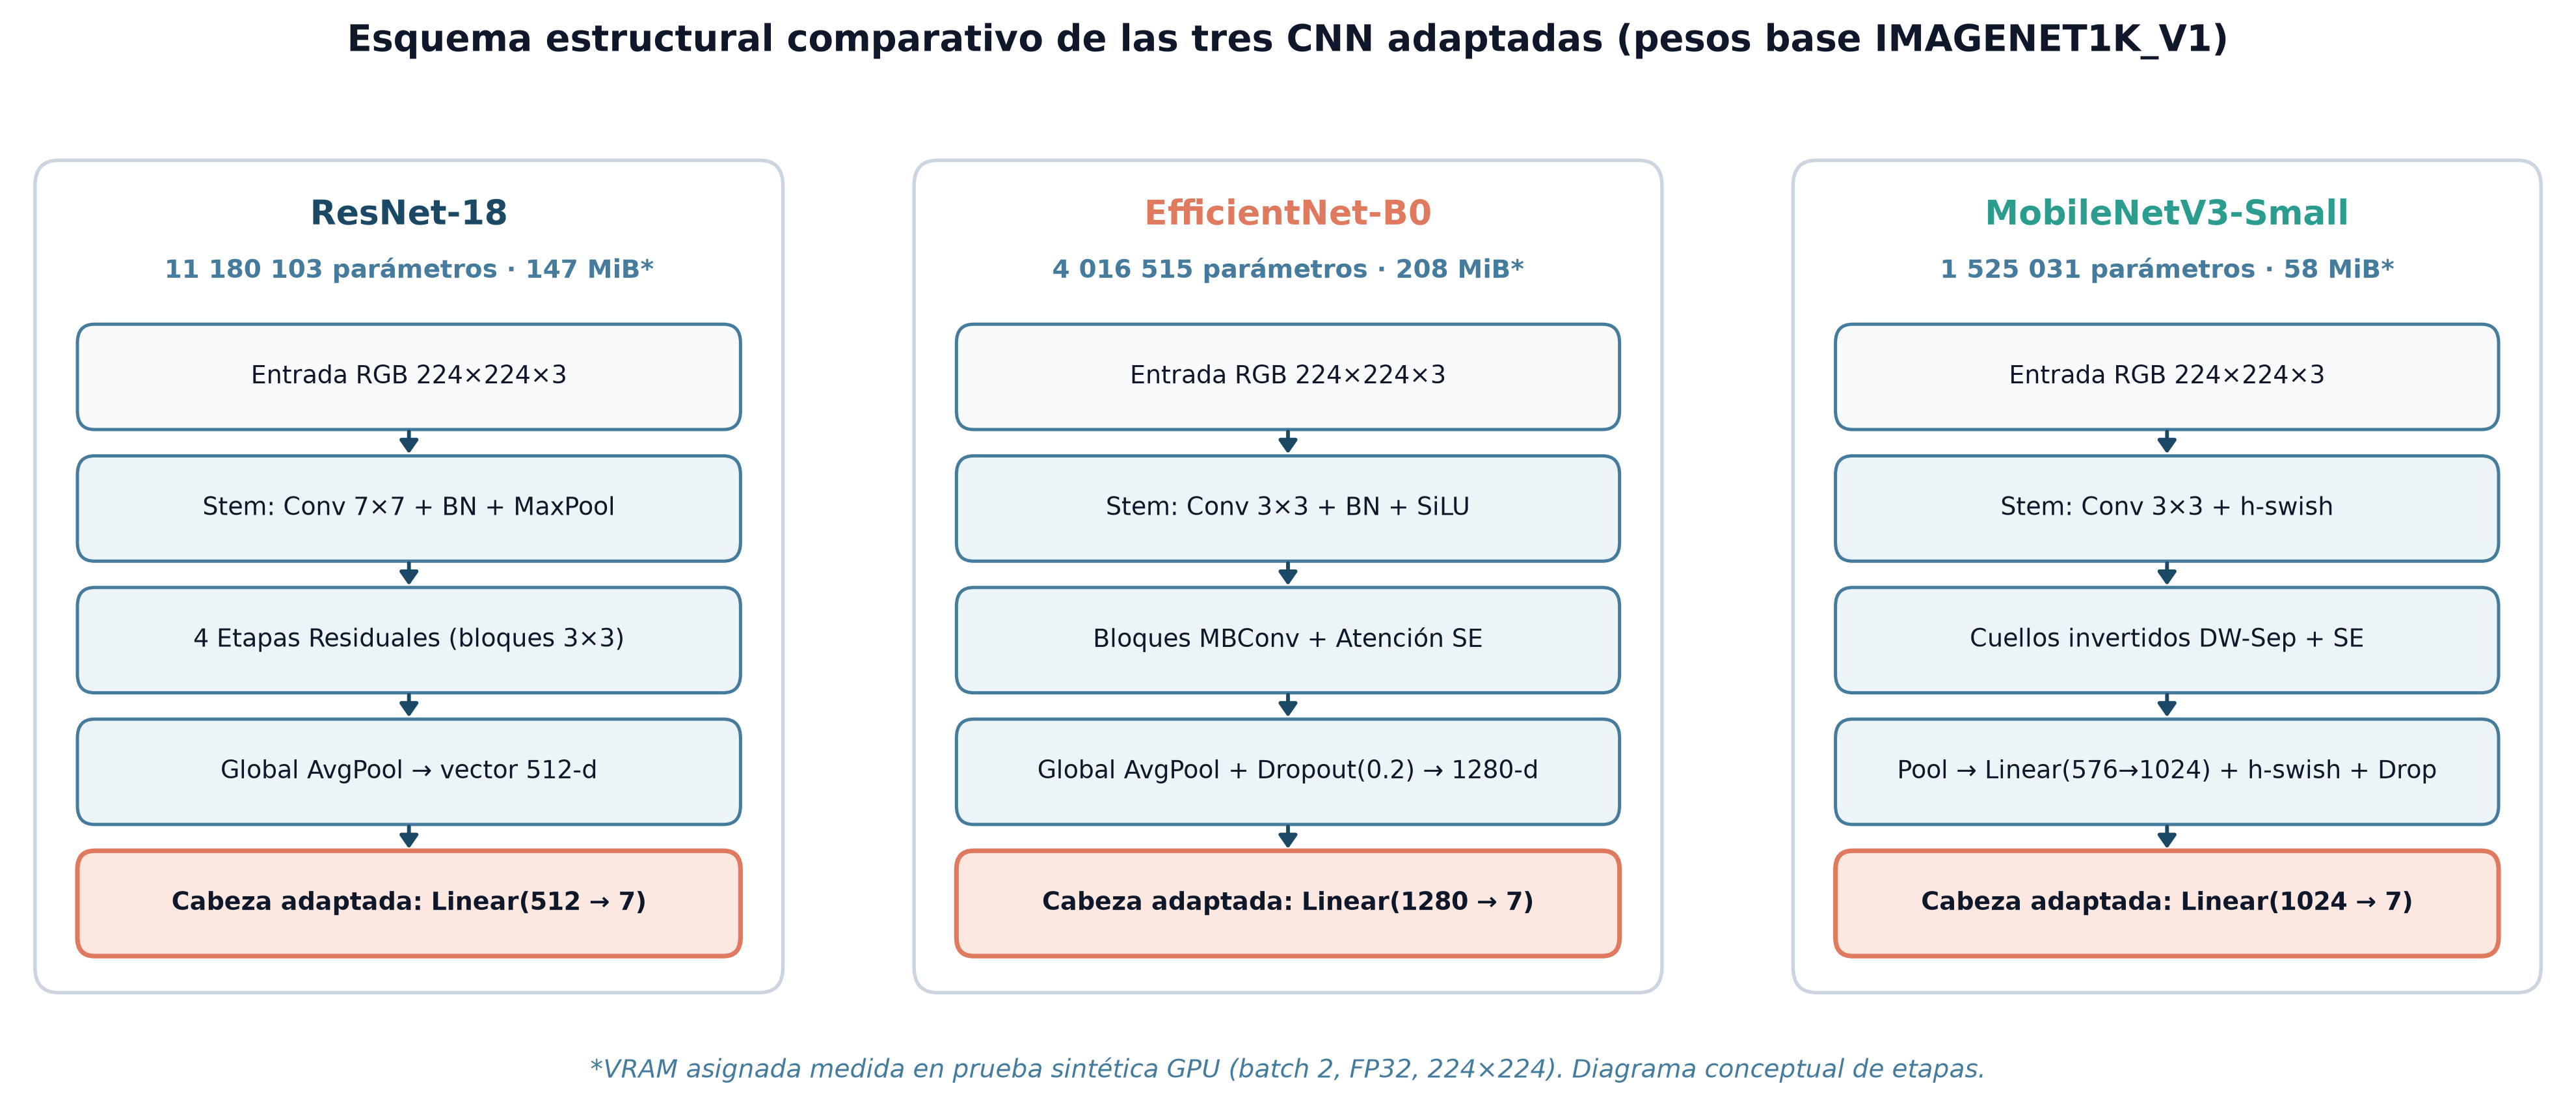
\includegraphics[width=0.96\textwidth,height=3.60cm,keepaspectratio]{11_arquitecturas.png}

  \vspace{0.18cm}
  \scriptsize
  \setlength{\tabcolsep}{4pt}
  \renewcommand{\arraystretch}{1.18}
  \begin{tabular*}{\textwidth}{@{\extracolsep{\fill}}>{\bfseries}l l c c l r r@{}}
    \toprule
    \rowcolor{azulSuave} \textbf{\color{azulInst}Arquitectura} & \textbf{\color{azulInst}Bloques base} & \textbf{\color{azulInst}Atención SE} & \textbf{\color{azulInst}Activación} & \textbf{\color{azulInst}Cabeza adaptada} & \textbf{\color{azulInst}Parámetros} & \textbf{\color{azulInst}Ratio} \\ \midrule
    ResNet-18 & Residuales $3\times 3$ & No & ReLU & \texttt{Linear(512 $\to$ 7)} & 11\,180\,103 (11.18M) & $7.33\times$ \\
    EfficientNet-B0 & MBConv compuesto & Sí & SiLU & \texttt{Linear(1280 $\to$ 7)} & 4\,016\,515 (4.02M) & $2.63\times$ \\
    MobileNetV3-Small & DW-Sep + cuello inv. & Sí & ReLU / h-swish & \texttt{Linear(1024 $\to$ 7)} & 1\,525\,031 (1.53M) & $1.00\times$ \\
    \bottomrule
  \end{tabular*}

  \vspace{0.14cm}
  {\scriptsize\color{grisTexto}\centering Mismo código en \texttt{models.py}, mismas ponderaciones iniciales \texttt{IMAGENET1K\_V1} y salida unificada a las 7 clases de HAM10000.\par}
\end{frame}

% ==============================================================================
% DIAPOSITIVA 6: PROTOCOLO HOMOGÉNEO Y ENTRENAMIENTO EN GTX 1650
% ==============================================================================
\begin{frame}{5. Protocolo homogéneo y entrenamiento en GTX 1650}
  \begin{columns}[T,onlytextwidth]
    \begin{column}{0.45\textwidth}
      \begin{beamercolorbox}[wd=\linewidth,sep=6pt]{block body}
        {\footnotesize\bfseries\color{azulInst}Configuración común (\texttt{configs/base.json})}
        \vspace{3pt}
        \scriptsize
        \begin{itemize}\setlength{\itemsep}{3.5pt}
          \item \textbf{Entorno único:} Acer Nitro AN515-45, NVIDIA GTX 1650 (4 GiB), driver 621.01, PyTorch 2.11.0+cu128, FP32, \texttt{batch=8}, \texttt{num\_workers=4}, \texttt{seed=42}.
          \item \textbf{Entrenamiento en 2 etapas:} 2 épocas de cabeza (extractor congelado, \texttt{BatchNorm} en \texttt{eval()}, LR $10^{-4}$) + hasta 18 épocas de ajuste fino (LR base $10^{-5}$, decaimiento coseno).
          \item \textbf{Regularización y estabilidad:} AdamW (\texttt{wd} $10^{-4}$), recorte de gradiente $L_2=1.0$, parada temprana paciencia 5.
          \item \textbf{Entropía cruzada ponderada (\texttt{train}):} $w_{\mathrm{df}}=12.52$, $w_{\mathrm{vasc}}=10.01$, $w_{\mathrm{mel}}=1.29$, $w_{\mathrm{nv}}=0.21$.
          \item \textbf{Alcance:} despliegue interactivo excluido por indicación docente.
        \end{itemize}
      \end{beamercolorbox}
    \end{column}
    \begin{column}{0.53\textwidth}
      {\footnotesize\bfseries\color{azulInst}Resumen real de entrenamiento (selección por Macro F1 en \texttt{val})}\par
      \vspace{0.15cm}
      \scriptsize
      \setlength{\tabcolsep}{2.5pt}
      \renewcommand{\arraystretch}{1.25}
      \noindent\begin{tabular*}{\linewidth}{@{\extracolsep{\fill}}>{\bfseries}l c c r r c@{}}
        \toprule
        \rowcolor{azulSuave} \textbf{\color{azulInst}Modelo} & \textbf{\color{azulInst}Ép.} & \textbf{\color{azulInst}Mejor} & \textbf{\color{azulInst}s / ép.} & \textbf{\color{azulInst}VRAM pico} & \textbf{\color{azulInst}Val F1} \\ \midrule
        ResNet-18 & 16 & ép.\ 11 & \textbf{127.5} & 434.2 MiB & 0.6927 \\
        EfficientNet-B0 & 20 & ép.\ 19 & 188.6 & 805.7 MiB & \textbf{0.7059} \\
        MobileNetV3-S & 19 & ép.\ 14 & 156.3 & \textbf{211.8 MiB} & 0.6213 \\
        \bottomrule
      \end{tabular*}

      \vspace{0.22cm}
      \begin{beamercolorbox}[wd=\linewidth,sep=6pt]{block body}
        {\scriptsize\bfseries\color{azulInst}Observaciones de convergencia y trazabilidad}
        \vspace{2pt}
        \scriptsize
        \begin{itemize}\setlength{\itemsep}{2.5pt}
          \item \textbf{Duración total:} 34.0 min (ResNet-18), 62.9 min (EfficientNet-B0) y 49.5 min (MobileNetV3-Small).
          \item \textbf{Parada temprana:} activada en ResNet-18 (ép.\ 16) y MobileNetV3-Small (ép.\ 19); EfficientNet-B0 agotó las 20 épocas.
          \item \textbf{Reproducibilidad:} \texttt{best.pt} congelado antes de desbloquear \texttt{test}.
        \end{itemize}
      \end{beamercolorbox}
    \end{column}
  \end{columns}
\end{frame}

% ==============================================================================
% DIAPOSITIVA 7: DESEMPEÑO GLOBAL EN TEST LIMPIO (PRECISIÓN Y EXACTITUD)
% ==============================================================================
\begin{frame}{6. Desempeño global en test limpio: comparación de precisión y exactitud}
  \centering
  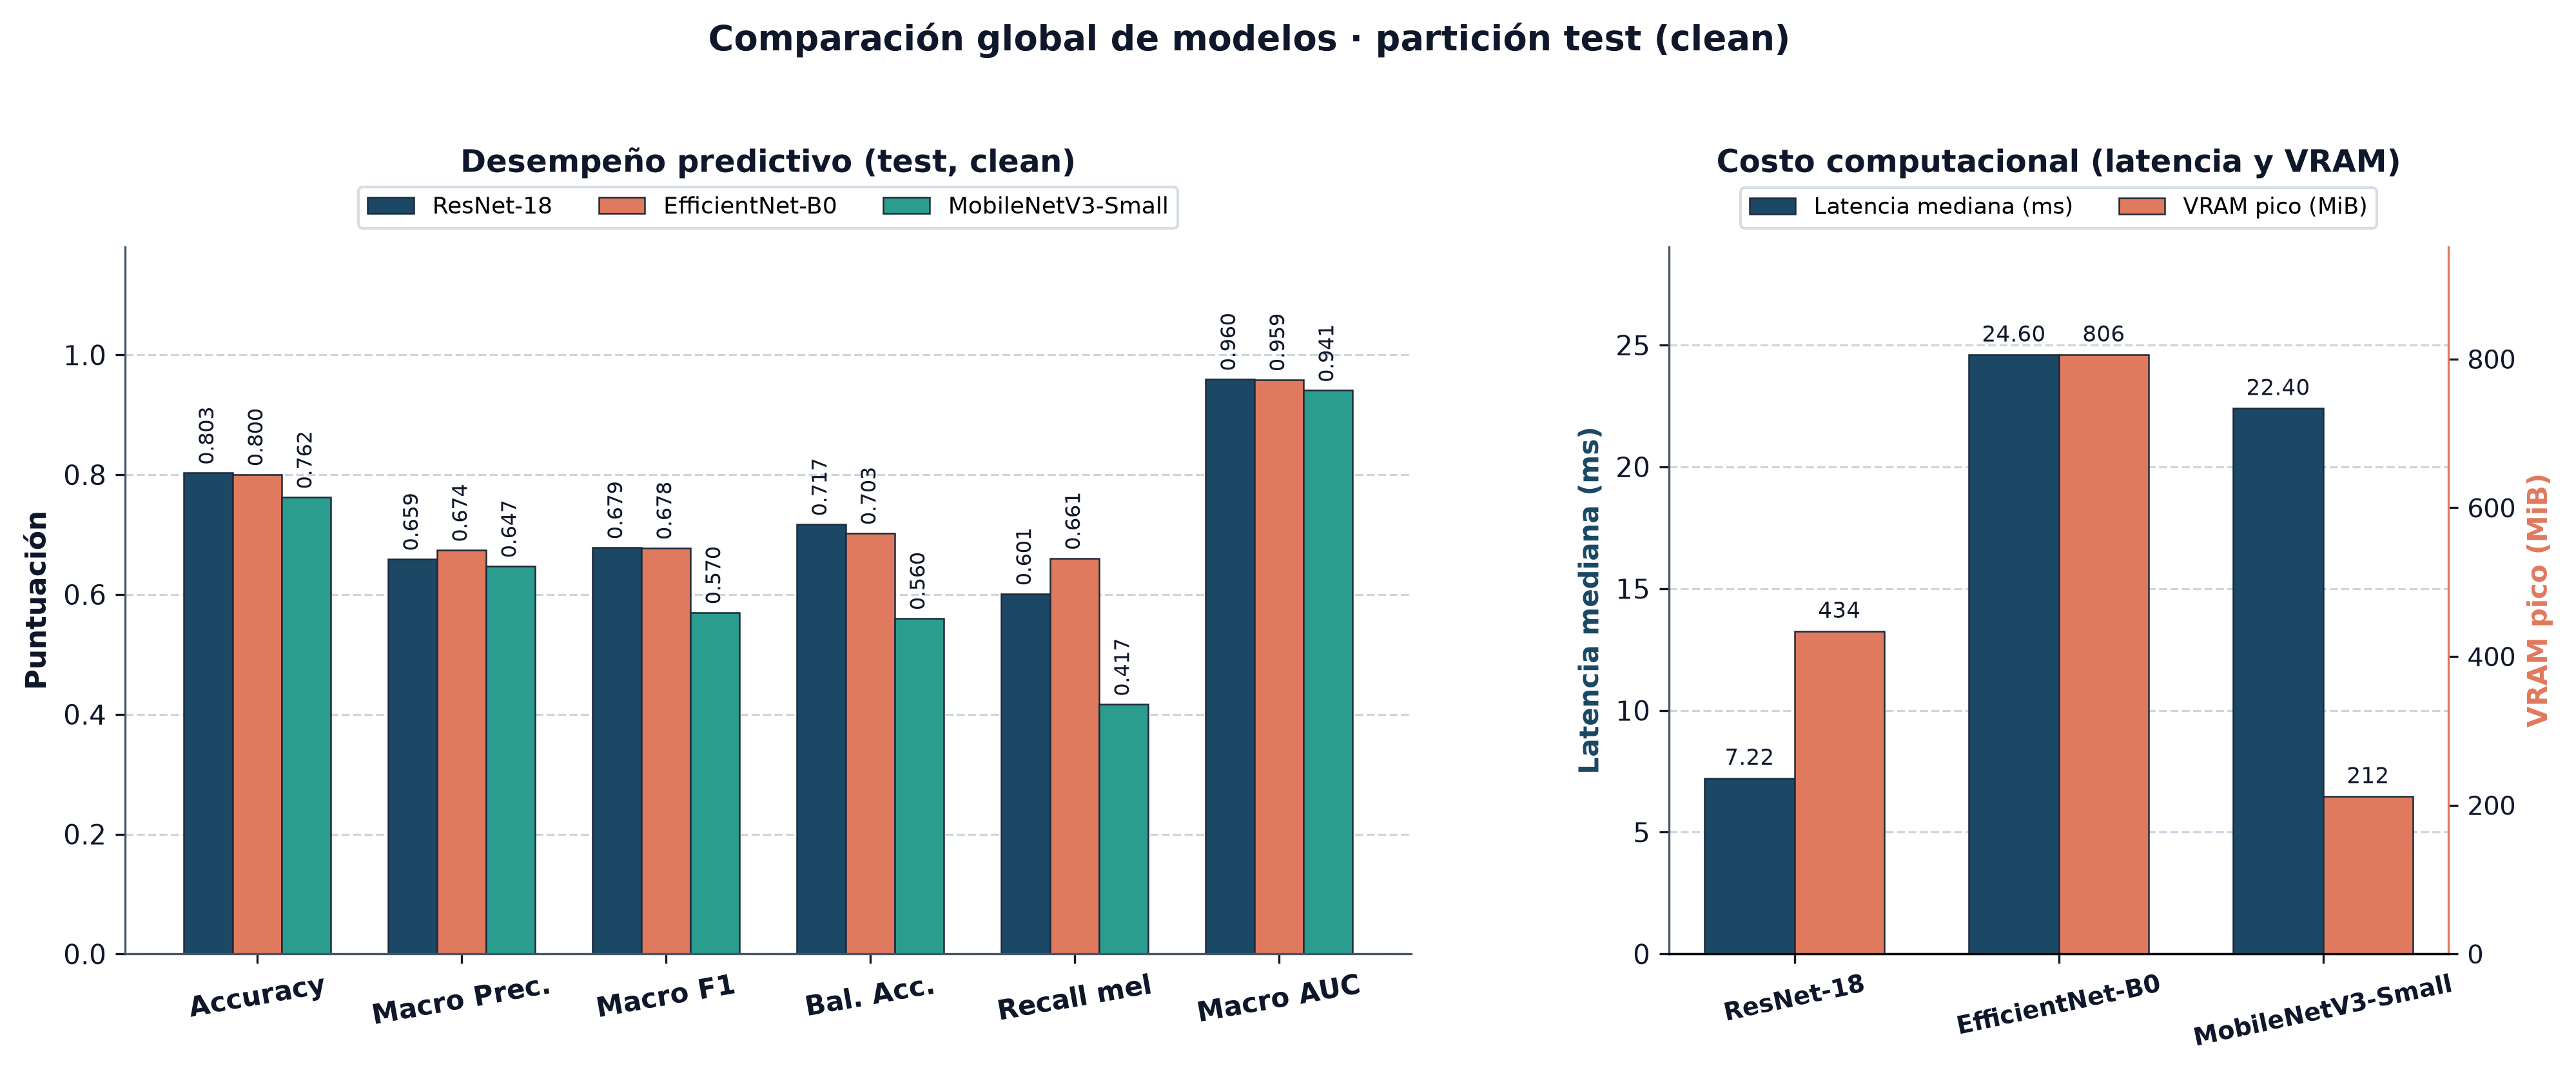
\includegraphics[width=0.98\textwidth,height=3.70cm,keepaspectratio]{comparacion_metricas.png}

  \vspace{0.10cm}
  \scriptsize
  \setlength{\tabcolsep}{3.0pt}
  \renewcommand{\arraystretch}{1.18}
  \begin{tabular*}{\textwidth}{@{\extracolsep{\fill}}>{\bfseries}l c >{\bfseries}c c c c c c@{}}
    \toprule
    \rowcolor{azulSuave} \textbf{\color{azulInst}Arquitectura} & \textbf{\color{azulInst}Accuracy} & \textbf{\color{naranjaAcc}Macro Prec.} & \textbf{\color{azulInst}Macro F1} & \textbf{\color{azulInst}Bal.\ Acc.} & \textbf{\color{azulInst}Recall \texttt{mel}} & \textbf{\color{azulInst}AUC OVR} & \textbf{\color{azulInst}Lat.\ \texttt{fwd} (P95) ms} \\ \midrule
    ResNet-18 & \textbf{0.8031} & 0.6591 & \textbf{0.6786} & \textbf{0.7174} & 0.6012 & \textbf{0.9596} & \textbf{7.22} (8.09) \\
    EfficientNet-B0 & 0.8004 & \textbf{\color{naranjaAcc}0.6741 (1.º)} & 0.6778 & 0.7025 & \textbf{0.6607} & 0.9587 & 24.60 (25.97) \\
    MobileNetV3-Small & 0.7625 & 0.6474 & 0.5700 & 0.5604 & 0.4167 & 0.9407 & 22.40 (23.97) \\
    \bottomrule
  \end{tabular*}

  \vspace{0.10cm}
  \begin{beamercolorbox}[wd=\linewidth,sep=4pt]{block body}
    {\scriptsize
    $\bullet$ \textbf{\color{naranjaAcc}Líder en Precisión ($TP/(TP+FP)$):} \textbf{EfficientNet-B0 lidera con 67.41\%} (frente a 65.91\% de ResNet-18 y 64.74\% de MobileNetV3-Small). Genera menos falsos positivos en queratosis actínica (\texttt{akiec}: 85.71\%) y nevus (\texttt{nv}: 92.97\%).\\
    $\bullet$ \textbf{\color{azulInst}Compromiso global de ResNet-18:} Lidera en \textbf{Exactitud (80.31\%)}, \textbf{Macro F1 (0.6786)} y \textbf{AUC (0.9596)}, con una inferencia \textbf{3.4$\times$ más veloz (7.22 ms vs.\ 24.60 ms)}.}
  \end{beamercolorbox}
\end{frame}

% ==============================================================================
% DIAPOSITIVA 8: CURVAS ROC Y MATRIZ DE CONFUSIÓN
% ==============================================================================
\begin{frame}{7. Curvas ROC comparativas y matriz de confusión (ResNet-18)}
  \begin{columns}[c,onlytextwidth]
    \begin{column}{0.61\textwidth}
      \centering
      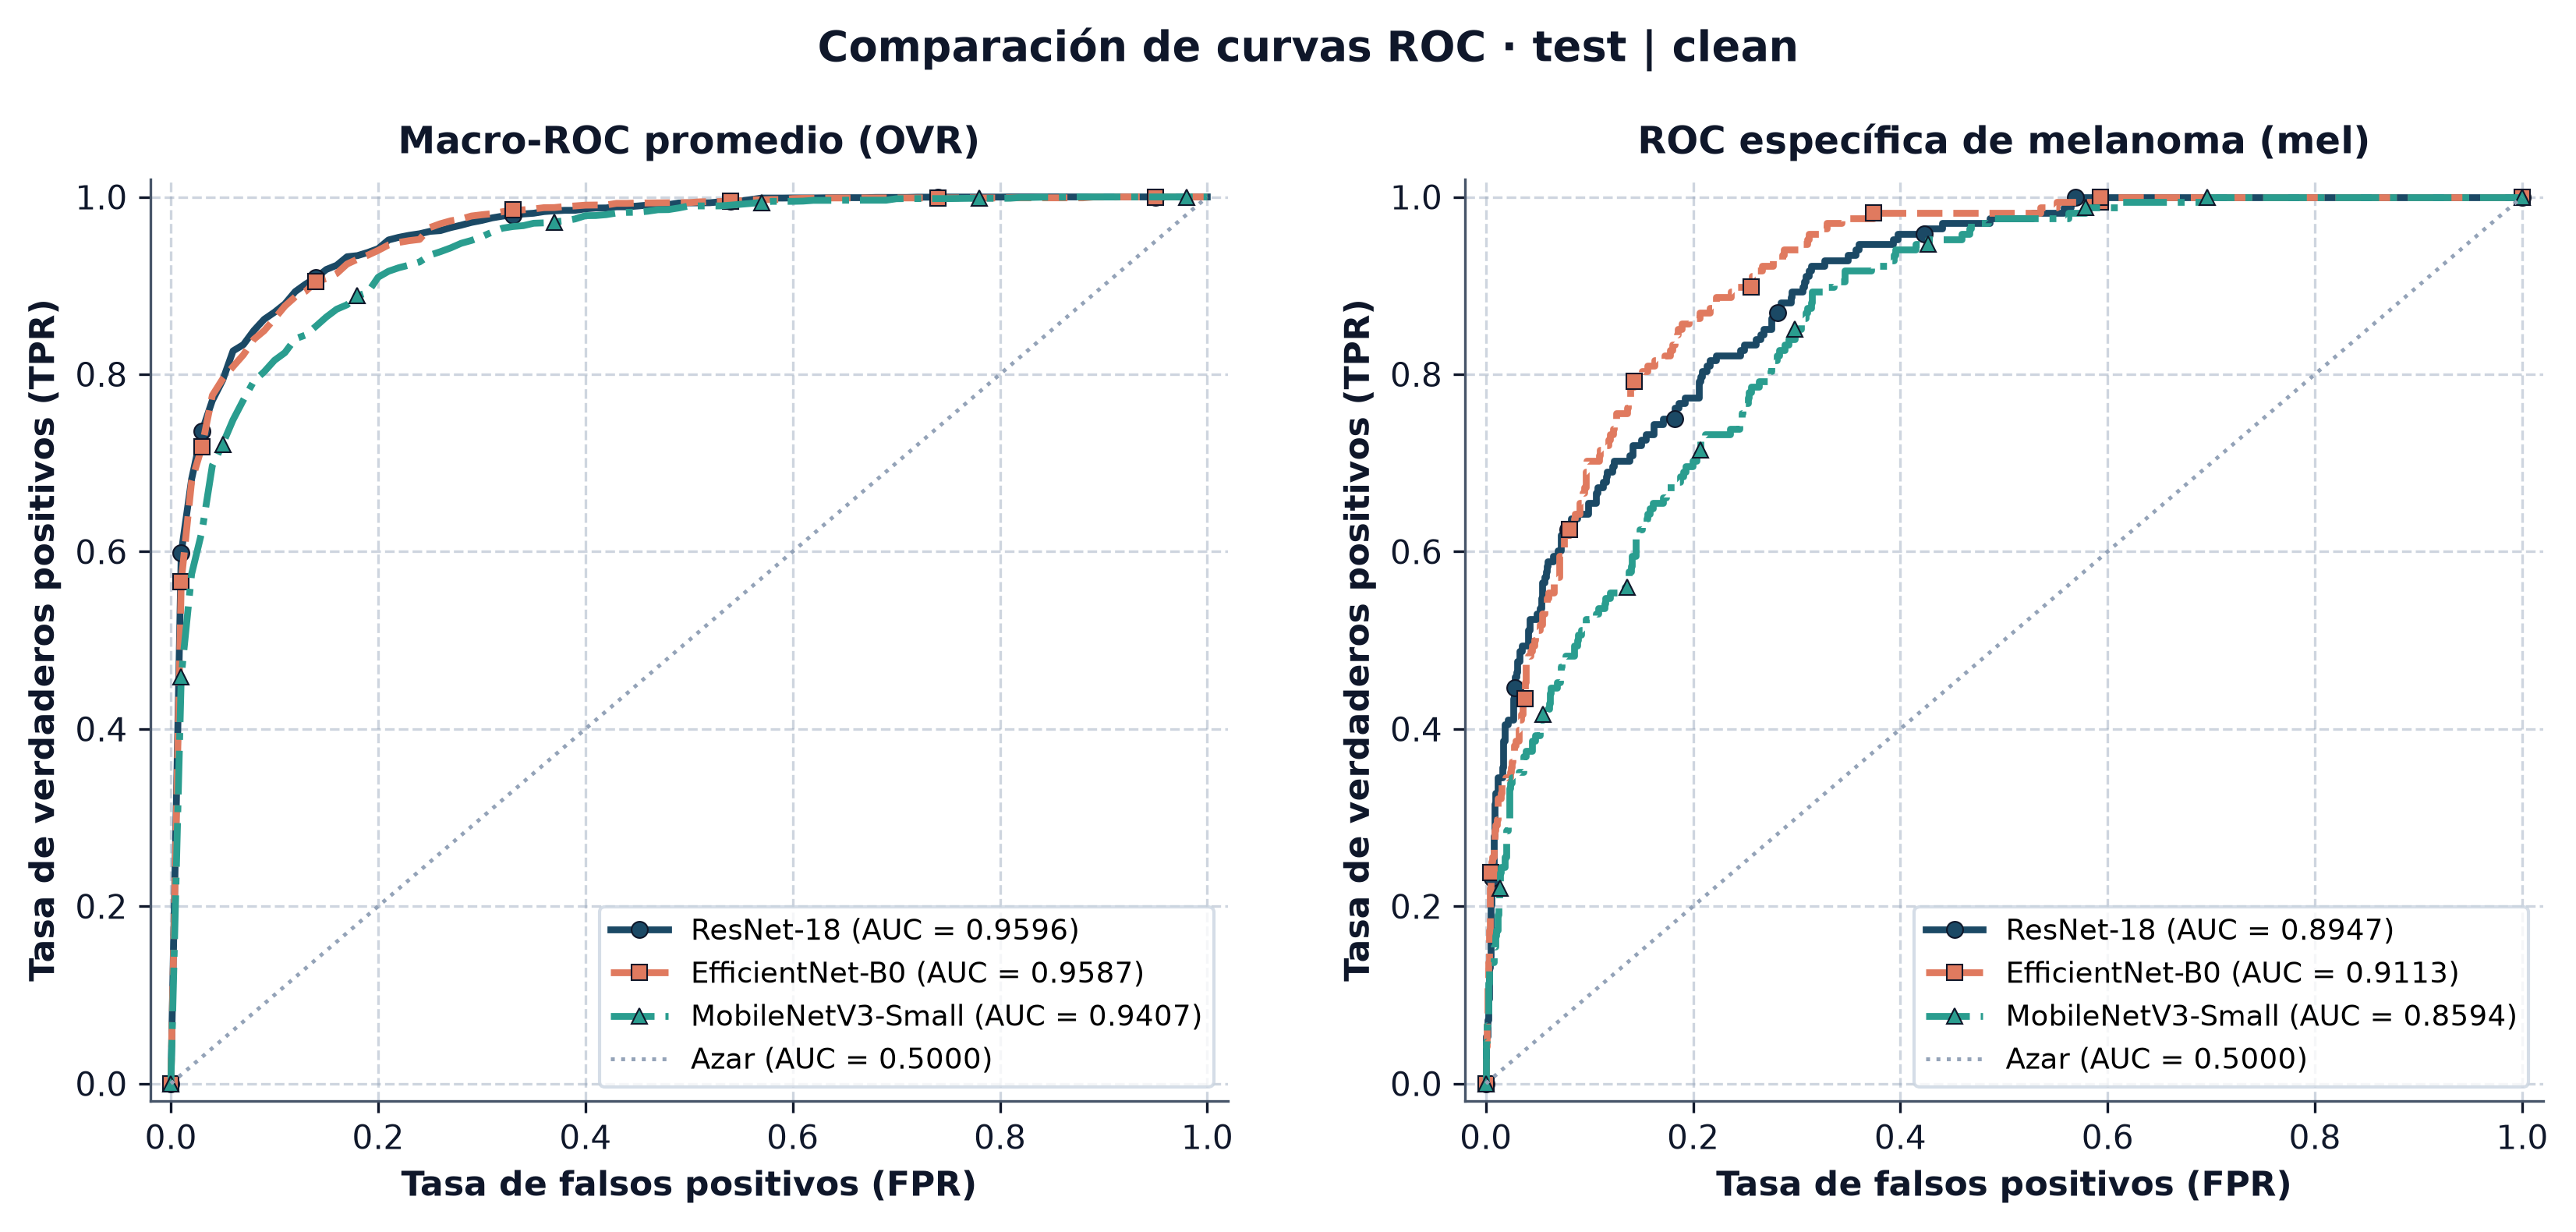
\includegraphics[width=\linewidth,height=4.20cm,keepaspectratio]{roc_comparativa_test_clean.png}
    \end{column}
    \begin{column}{0.37\textwidth}
      \centering
      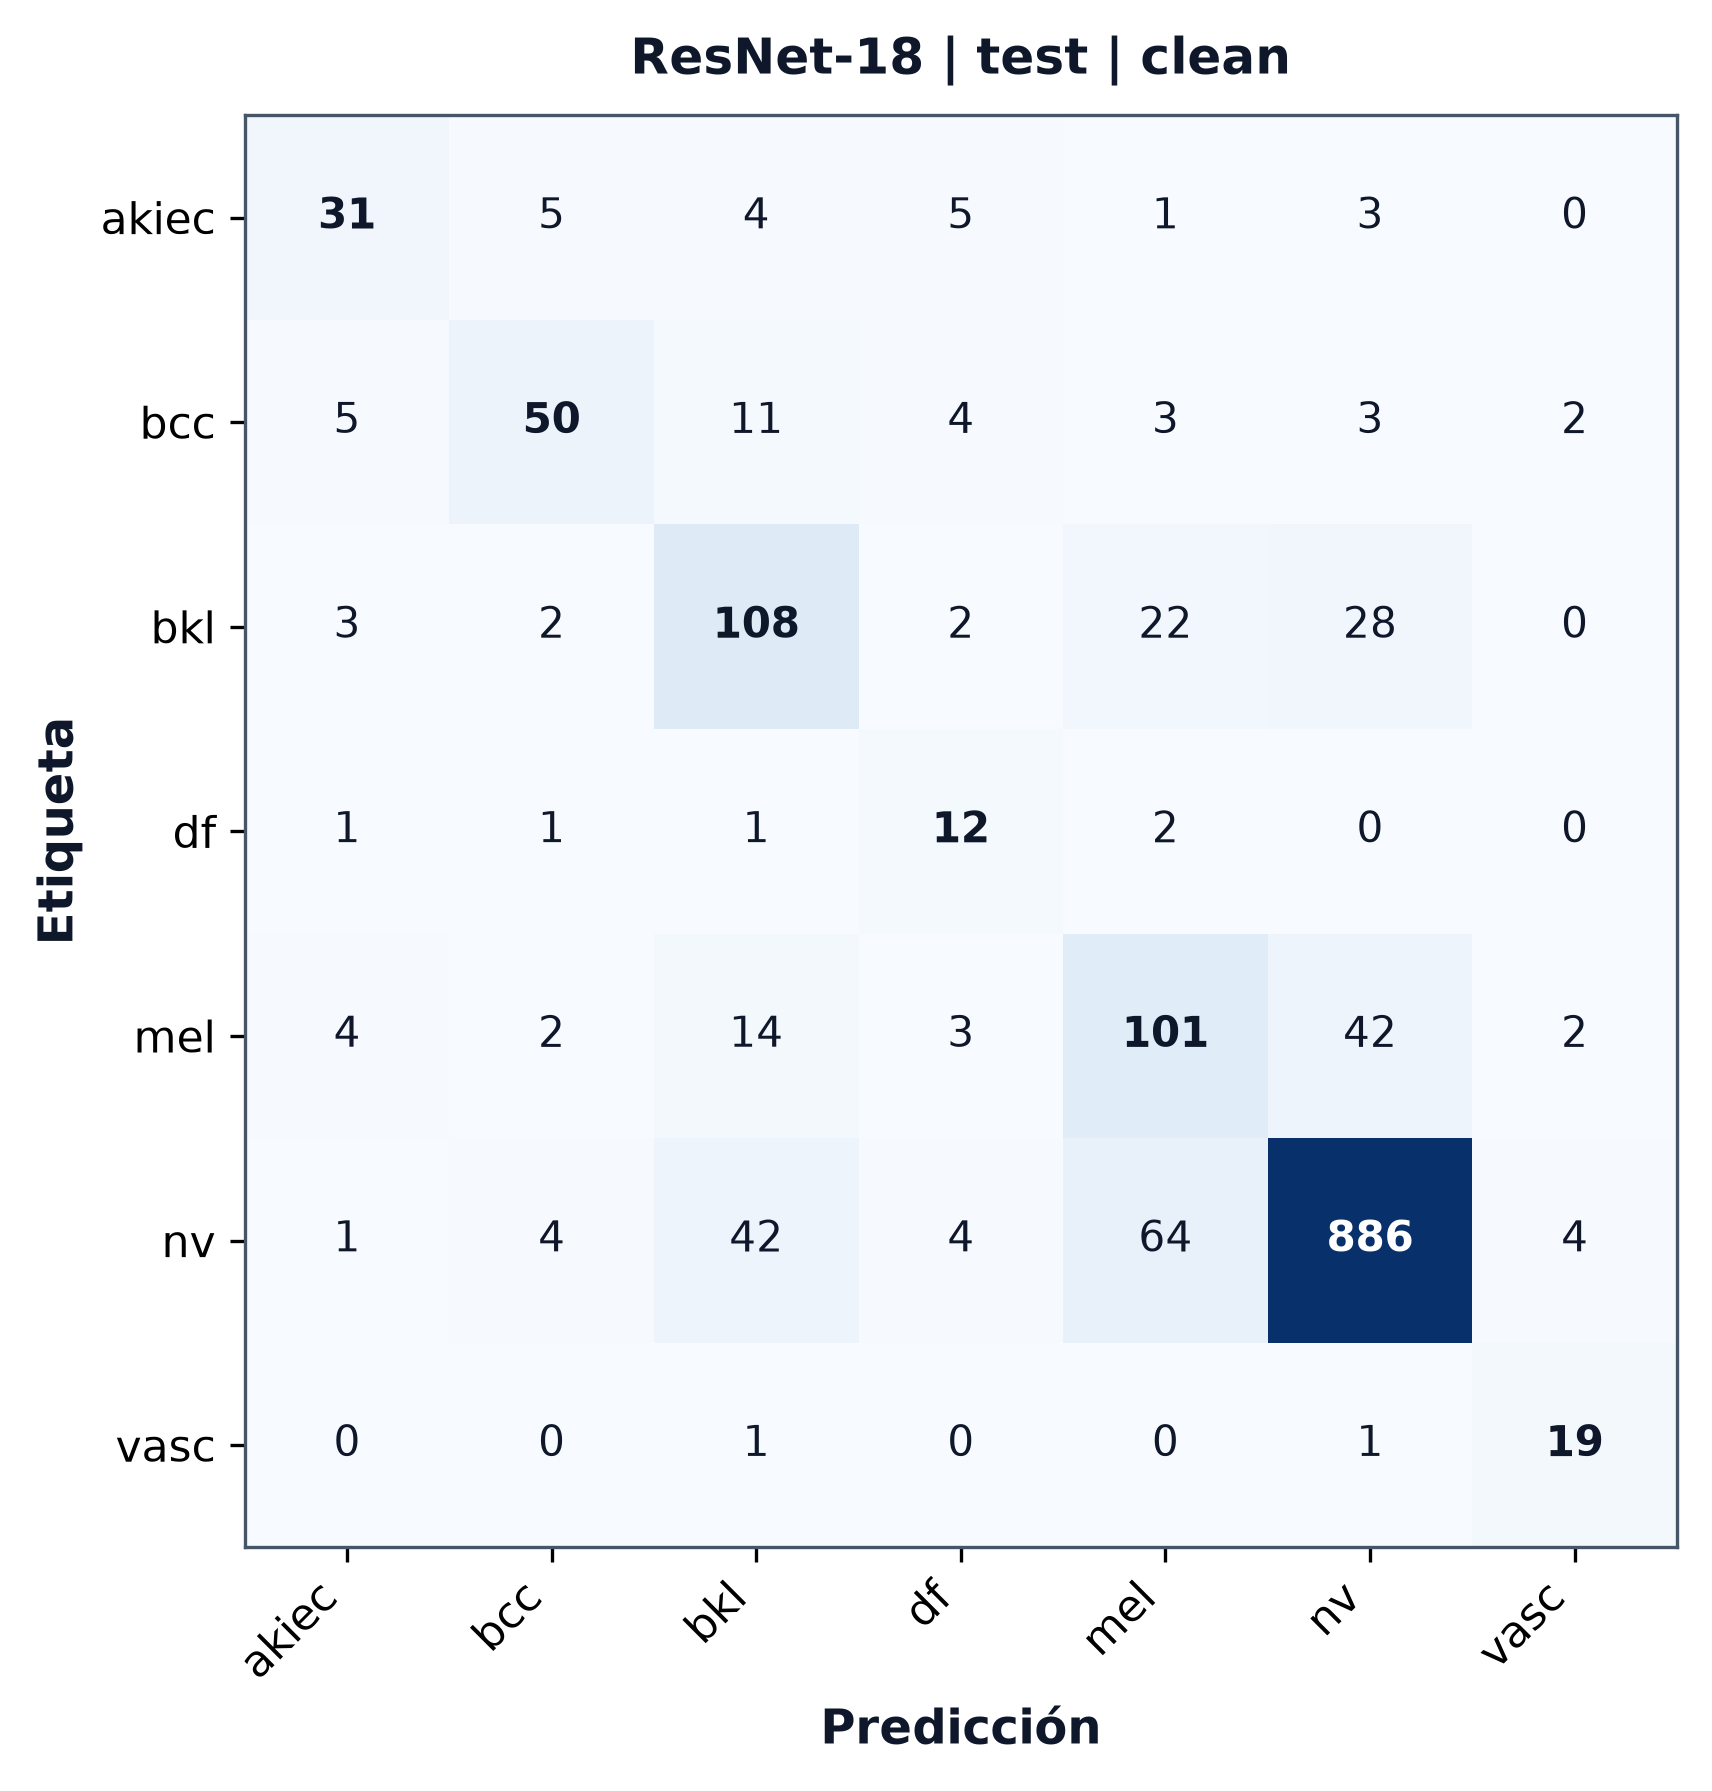
\includegraphics[width=\linewidth,height=4.20cm,keepaspectratio]{confusion_resnet18_42_test_clean.png}
    \end{column}
  \end{columns}

  \vspace{0.18cm}
  \begin{columns}[T,onlytextwidth]
    \begin{column}{0.61\textwidth}
      \tarjetainf{Discriminación ROC OVR y melanoma (\texttt{mel}, $n=168$)}{%
        \textbf{Macro-AUC} sólido en las tres redes (0.9596, 0.9587, 0.9407). En \texttt{mel}, \textbf{EfficientNet-B0} logra mayor AUC específico (0.911) y Recall \textbf{0.6607} (111/168), superando a ResNet-18 (AUC 0.895, Recall \textbf{0.6012}, 101/168) y MobileNetV3-Small (AUC 0.859, Recall \textbf{0.4167}).}
    \end{column}
    \begin{column}{0.37\textwidth}
      \tarjetainf{Errores en matriz de ResNet-18}{%
        Fuerte acierto en \texttt{nv} (886/1\,005) y \texttt{vasc} (19/21). La confusión principal ocurre entre \texttt{mel}, \texttt{nv} y \texttt{bkl} (42 \texttt{mel}$\to$\texttt{nv}; 64 \texttt{nv}$\to$\texttt{mel}).}
    \end{column}
  \end{columns}
\end{frame}

% ==============================================================================
% DIAPOSITIVA 9: SENSIBILIDAD AL RUIDO/DESENFOQUE Y MITIGACIÓN ESPACIAL
% ==============================================================================
\begin{frame}{8. Sensibilidad a ruido/desenfoque y mitigación espacial en \texttt{test}}
  \centering
  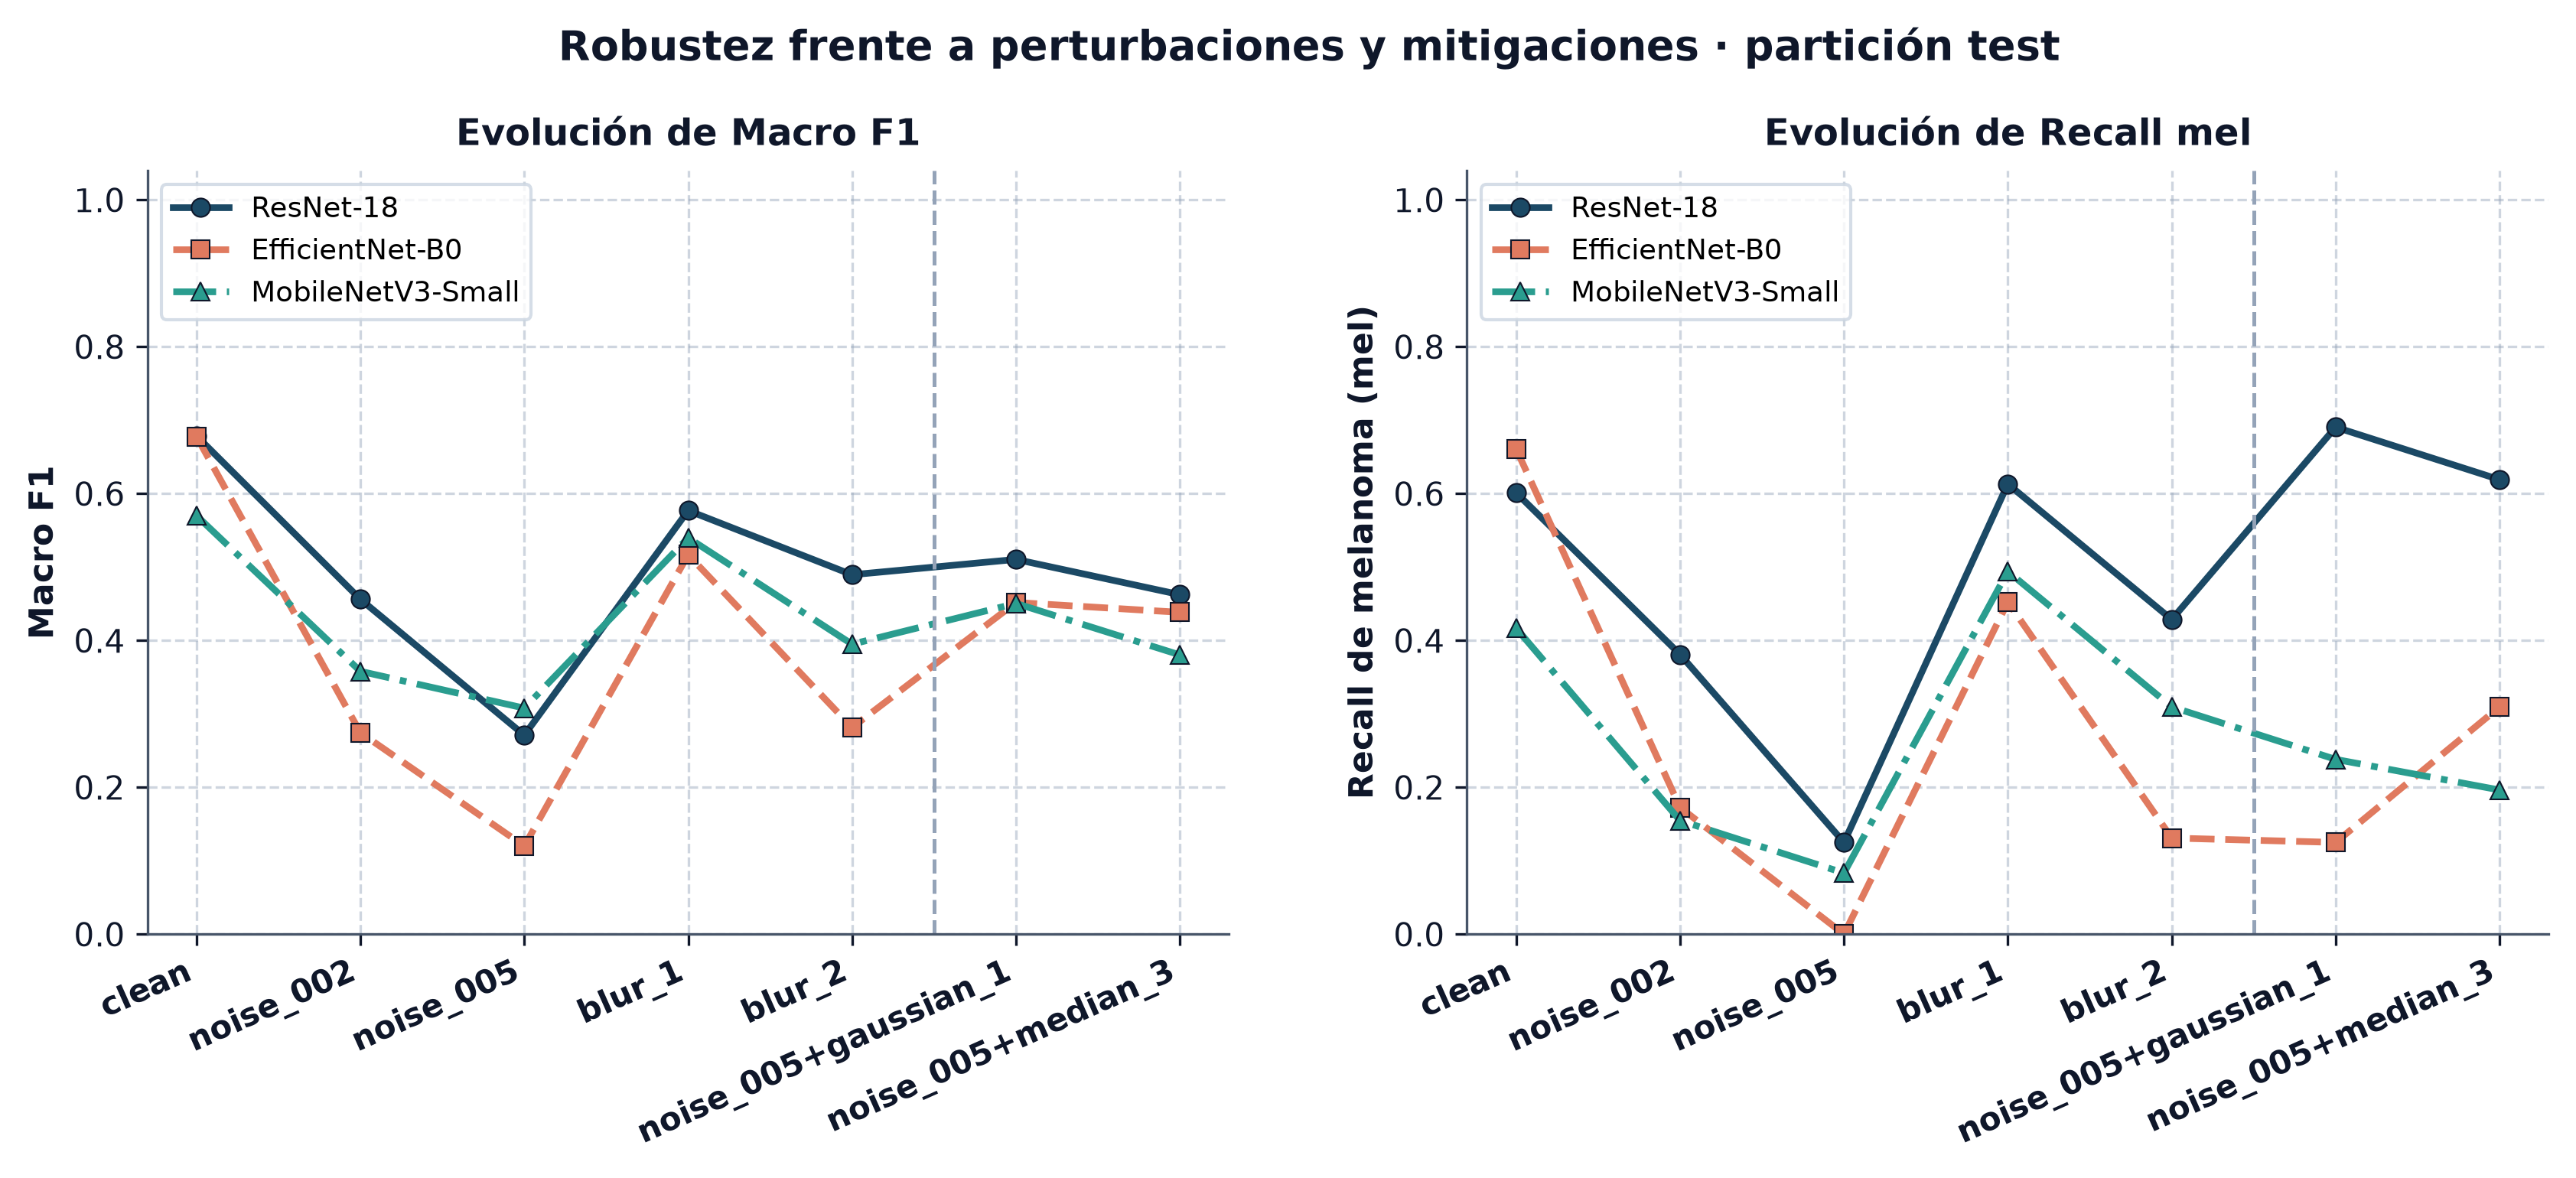
\includegraphics[width=0.95\textwidth,height=3.60cm,keepaspectratio]{comparacion_robustez.png}

  \vspace{0.15cm}
  \scriptsize
  \renewcommand{\arraystretch}{1.18}
  \setlength{\tabcolsep}{3pt}
  \begin{tabular*}{\textwidth}{@{\extracolsep{\fill}}>{\bfseries}l c c c c c | c c@{}}
    \toprule
    \rowcolor{azulSuave} \textbf{\color{azulInst}Arquitectura (Macro F1)} & \textbf{\color{azulInst}\texttt{clean}} & \textbf{\color{azulInst}\texttt{noise\_002}} & \textbf{\color{azulInst}\texttt{noise\_005}} & \textbf{\color{azulInst}\texttt{blur\_1}} & \textbf{\color{azulInst}\texttt{blur\_2}} & \textbf{\color{azulInst}+ \texttt{median\_3}} & \textbf{\color{azulInst}+ \texttt{gaussian\_1}} \\ \midrule
    ResNet-18 & \textbf{0.6786} & \textbf{0.4561} & 0.2710 & \textbf{0.5769} & \textbf{0.4895} & \textbf{0.4624} {\tiny (mel 0.619)} & \textbf{0.5104} {\tiny (mel \textbf{0.691})} \\
    EfficientNet-B0 & 0.6778 & 0.2745 & 0.1201 {\tiny (mel \textbf{0.000})} & 0.5167 & 0.2815 & 0.4383 {\tiny (mel 0.310)} & 0.4518 {\tiny (mel 0.125)} \\
    MobileNetV3-Small & 0.5700 & 0.3580 & \textbf{0.3079} {\tiny (mel 0.083)} & 0.5398 & 0.3949 & 0.3804 {\tiny (mel 0.196)} & 0.4505 {\tiny (mel 0.238)} \\
    \bottomrule
  \end{tabular*}

  \vspace{0.12cm}
  \begin{beamercolorbox}[wd=\linewidth,sep=4pt]{block body}
    \centering\scriptsize
    \textbf{\color{azulInst}Hallazgo crítico:} EfficientNet-B0 colapsa en \texttt{noise\_005} (F1 \textbf{0.1201}, Rec.\ \texttt{mel} \textbf{0.0000}). \texttt{gaussian\_1} aporta \textbf{+0.14 a +0.33} pts de Macro F1; en ResNet-18 sube Rec.\ \texttt{mel} (\textbf{0.6012 $\to$ 0.6905}), pero baja Prec.\ \texttt{mel} (\textbf{0.5233 $\to$ 0.3648}; 92 $\to$ 202 FP): mitigación parcial.
  \end{beamercolorbox}
\end{frame}

% ==============================================================================
% DIAPOSITIVA 10: EFICIENCIA GPU (POR QUÉ RESNET-18 ES MÁS RÁPIDO EN BATCH=1)
% ==============================================================================
\begin{frame}{9. Eficiencia GPU: \texttt{forward()} \texttt{batch=1} y posibles factores}
  \scriptsize
  \setlength{\tabcolsep}{3.5pt}
  \renewcommand{\arraystretch}{1.20}
  \begin{tabular*}{\textwidth}{@{\extracolsep{\fill}}>{\bfseries}l c c c c c@{}}
    \toprule
    \rowcolor{azulSuave} \textbf{\color{azulInst}Arquitectura} & \textbf{\color{azulInst}Parámetros} & \textbf{\color{azulInst}VRAM pico (train)} & \textbf{\color{azulInst}Tiempo / época} & \textbf{\color{azulInst}Lat.\ \texttt{fwd} limpio (rango)} & \textbf{\color{azulInst}Factor vs.\ ResNet-18} \\ \midrule
    ResNet-18 & 11.18 M & 434.2 MiB & \textbf{127.5 s} & \textbf{7.22 ms} (6.86--9.46) & $1.00\times$ (referencia) \\
    MobileNetV3-Small & \textbf{1.53 M} & \textbf{211.8 MiB} & 156.3 s & 22.40 ms (15.26--22.40) & $3.10\times$ más lento \\
    EfficientNet-B0 & 4.02 M & 805.7 MiB & 188.6 s & 24.60 ms (22.49--34.82) & $3.41\times$ más lento \\
    \bottomrule
  \end{tabular*}

  \vspace{0.22cm}
  \begin{columns}[T,onlytextwidth]
    \begin{column}{0.32\textwidth}
      \begin{beamercolorbox}[wd=\linewidth,sep=6pt]{block body}
        {\footnotesize\bfseries\color{azulInst}Hipótesis 1: Kernels CUDA}\\[3pt]
        \scriptsize
        MobileNetV3-Small (7.3$\times$ menos parámetros) fragmentaría cada bloque en múltiples micro-operaciones ($1\times 1$, \emph{depthwise}, SE), aumentando el despacho CPU$\to$GPU en \texttt{batch=1} FP32.
      \end{beamercolorbox}
    \end{column}
    \begin{column}{0.32\textwidth}
      \begin{beamercolorbox}[wd=\linewidth,sep=6pt]{block body}
        {\footnotesize\bfseries\color{azulInst}Hipótesis 2: Intensidad}\\[3pt]
        \scriptsize
        Las convoluciones \emph{depthwise} tendrían menor reutilización en caché (\emph{memory-bound}), mientras las densas $3\times 3$ de ResNet-18 aprovecharían mejor los núcleos optimizados de \textbf{cuDNN}.
      \end{beamercolorbox}
    \end{column}
    \begin{column}{0.32\textwidth}
      \begin{beamercolorbox}[wd=\linewidth,sep=6pt]{block body}
        {\footnotesize\bfseries\color{azulInst}Hipótesis 3: SE y VRAM}\\[3pt]
        \scriptsize
        La atención SE y activaciones (\texttt{h-swish}, \texttt{SiLU}) añadirían accesos a memoria global; las expansiones en EfficientNet-B0 elevan la VRAM de entrenamiento a \textbf{805.7 MiB}.
      \end{beamercolorbox}
    \end{column}
  \end{columns}

  \vspace{0.20cm}
  \begin{beamercolorbox}[wd=\linewidth,sep=5pt]{block body}
    \centering\scriptsize
    \textbf{\color{azulInst}Alcance de medición:} La latencia mide solo \texttt{forward()} en GPU (\texttt{batch=1}, sin E/S ni filtrado en CPU); las explicaciones son hipótesis interpretativas sin perfilado por kernel.
  \end{beamercolorbox}
\end{frame}

% ==============================================================================
% DIAPOSITIVA 11: LIMITACIONES, CONCLUSIONES Y VEREDICTO FINAL
% ==============================================================================
\begin{frame}{10. Limitaciones, conclusiones y veredicto final}
  \begin{columns}[T,onlytextwidth]
    \begin{column}{0.49\textwidth}
      \begin{beamercolorbox}[wd=\linewidth,sep=6pt]{block body}
        {\footnotesize\bfseries\color{azulInst}Limitaciones y validez del estudio}
        \vspace{3pt}
        \scriptsize
        \begin{itemize}\setlength{\itemsep}{3pt}
          \item \textbf{Sin \texttt{patient\_id}:} \texttt{HAM10000\_metadata.csv} identifica lesiones, no pacientes; dos lesiones de una persona podrían separarse.
          \item \textbf{Test interno y sesgo demográfico:} colección mayoritariamente de piel clara; no sustituye validación multicéntrica externa.
          \item \textbf{Varianza y semilla única:} \texttt{df} ($n=17$) y \texttt{vasc} ($n=21$) en \texttt{test} tienen alta varianza; evaluado con \texttt{seed=42}.
          \item \textbf{Uso estrictamente académico:} no constituye producto médico; despliegue web/móvil excluido por indicación docente.
        \end{itemize}
      \end{beamercolorbox}
    \end{column}
    \begin{column}{0.49\textwidth}
      \begin{beamercolorbox}[wd=\linewidth,sep=6pt]{block body}
        {\footnotesize\bfseries\color{azulInst}Conclusiones principales}
        \vspace{3pt}
        \scriptsize
        \begin{itemize}\setlength{\itemsep}{3pt}
          \item Se consolidó un flujo reproducible con \textbf{0 fugas} de lesión o SHA-256 entre 10\,015 imágenes (\texttt{split\_sha256} verificado).
          \item Las tres CNN alcanzan AUC OVR $>0.94$ en limpio sobre GPU de 4 GiB, con Macro Prec.\ de 0.6474--0.6741.
          \item El ruido \texttt{noise\_005} colapsa a EfficientNet-B0; \texttt{gaussian\_1} logra \textbf{mitigación parcial} ($+0.14$ a $+0.33$ Macro F1), pero eleva FP en melanoma ($92 \to 202$ en ResNet-18).
          \item En \texttt{forward()} \texttt{batch=1} en GTX 1650, ResNet-18 fue 3.1--3.4$\times$ más rápida en limpio (6.86--9.46 ms entre corridas).
        \end{itemize}
      \end{beamercolorbox}
    \end{column}
  \end{columns}

  \vspace{0.20cm}
  \begin{beamercolorbox}[wd=\linewidth,sep=6pt]{frametitle}
    {\footnotesize\bfseries VEREDICTO FINAL · MEJOR BALANCE OBSERVADO: RESNET-18}\\[2pt]
    {\scriptsize Sin superioridad estadística en Macro F1 frente a EfficientNet-B0 ($\Delta=0.00084$; IC95\% $[-0.0429,+0.0464]$), ResNet-18 ofrece el mejor balance observado en este protocolo y GTX 1650: mayor \textbf{Bal.\ Acc.\ (0.7174)}, \textbf{AUC OVR (0.9596)}, menor latencia \texttt{forward()} (\textbf{7.22 ms}) y mejor respuesta parcial con \texttt{gaussian\_1}. EfficientNet-B0 lidera en Macro Prec.\ (\textbf{0.6741}) y Rec.\ \texttt{mel} limpio (\textbf{0.6607}), pero colapsa en \texttt{noise\_005}.}
  \end{beamercolorbox}
\end{frame}

\end{document}
